\documentclass[a4paper]{report}
 
%PhD Thesis Template for the School of Electronic Engineering and Computer Science, Queen Mary University of London. Stripped from Dan Stowell's PhD.

%BEFORE SUBMISSION DO THESE:
% * deactivate all \includeonly
% * ensure \doneit set to nothing
% * ensure numbering CONTINUOUS from title page on through
% * activate the includes of license, ack, etc
% * check through for question mark errors in render
% * make sure the bibliog doesn't have ugly urls in

\usepackage[dvipsnames]{xcolor}
\usepackage{ifdraft}
\usepackage{amsmath}
\usepackage{amsfonts}
\usepackage{amssymb}
\usepackage{natbib}
\usepackage{rotating}
\usepackage{hyperref}
\usepackage{subfig} % apparently subfig is the one to use not subfigure
\usepackage{appendix}
\usepackage{tipa}
\usepackage{clrscode}
\usepackage{setspace}
\usepackage[absolute]{textpos} 
\usepackage{caption}
\usepackage{tikz}
\usetikzlibrary{shapes,arrows}

\usepackage{xurl}
% \usepackage{times}
\usepackage{soul,color}
\usepackage{graphicx}
\usepackage{natbib}
\usepackage{flushend}

\begin{document}

\setlength{\TPHorizModule}{200mm} 
\setlength{\TPVertModule}{100mm} 
\textblockorigin{61mm}{19mm}
\renewcommand{\baselinestretch}{2}

%%%%% thanks alex mclean for super-useful onscreen reading tip:
%\usepackage[top=0.1in, bottom=0.1in, left=0.3in, right=0.3in, paperwidth=11in, paperheight=7in]{geometry} % activate for ONSCREEN reading shape AT HOME
%\usepackage[top=0.1in, bottom=0.1in, left=0.3in, right=0.3in, paperwidth=11in, paperheight=8.5in]{geometry} % activate for ONSCREEN reading shape AT WORK

\onehalfspacing{}

% activate the appropriate shortcut, whether or not to show this in titles
%	\providecommand{\doneit}{DONE: }
%	\providecommand{\doneit}{}

% Some specific notations used:
\providecommand{\OT}[1]{\operatorname{\Theta}\bigl(#1\bigr)}
\providecommand{\OOm}[1]{\operatorname{\Omega}\bigl(#1\bigr)}
%\newcommand{\concat}{{\,++\,}}

% numbering starts from here:
\pagenumbering{arabic}

% titlepage stuff
\title{\textit{Expanding the Generative Space}: Data-Free Techniques for Active Divergence with Generative Neural Networks}
% \title{Active Divergence with Generative Deep Learning: Methods, Metrics and Taxonomies}
\author{Terence Broad \\
\\
\\
\\
A dissertation submitted in partial satisfaction \\
of the requirements for the degree\\
 Doctor of Philosophy\\
\\
\\
\\
Department of Computing\\
Goldsmiths, University of London
}


\date{2024}

\maketitle
% qmul rules say abstract must be FIRST after title page

\begin{abstract}

tbc

\end{abstract}  

\setcounter{page}{3}

% \chapter*{Acknowledgements}

First and foremost I would like to thank my supervisors Professor Mick Grierson and Professor Frederic Fol Leymarie for their dedicated support over the long journey of this research and my prior academic training, and to the wider community of academics in the department of Computing at Goldsmiths who supported me over my many years there. I will be eternally grateful to those at Goldsmiths who had the dedication and vision to establish Creative Computing as an academic discipline and create a place for people like me to thrive in. 

I would like to thank Professor Rebecca Fiebrink and Professor Matthew Yee-King for the invaluable feedback in my upgrade examination, which massively influenced the final shape of this thesis. Additionally, I would like to thank the examiners of this PhD, Professor Phillipe Pasquier and Professor Marco Gillies, for their time and the thoughtful questions they prepared for what was a very enjoyable viva. 

I would like to thank my friend and PhD colleague Sebastian Berns for coining the term \textit{active divergence} that succinctly defined and tied together what I had thought were very disparate pieces of research when I had originally conducted them. I would like to thank the principal investigators, admin team and the other fellow students from the Centre for Doctoral Training in Intelligent Games and Game Intelligence (IGGI; grant EP/L015846/1) for providing the support and community to make this PhD possible. I would also like to thank Sara Bodinar and Jan Birley from Writers Retreat UK for providing the space and mentorship during my retreat there in 2023 where the final framing and narrative of this thesis took shape. 

I would like to thank the curators and other organisers who chose to exhibit and showcase artworks made during this thesis, which include Luba Elliot, Xavier Snelgrove, Gemma Murray, Susanna Pousette, Paula Perissinotto, Clarissa Oliveira, Mathieu Arbez Hermoso and Rita Hajj. I would also like to thank Georgie Hoare, Joe Bedell-Brill from the band 0171 to use their commission as a test-bed for some of this research and document that process in this thesis.

I would like to thank my good friend Joe for his generosity and support during the first COVID lockdown and the support he gave to this research during that pivotal time. I would like to thank my partner Katie, for her patience and the resolute support that I so desperately needed in the final stages of this PhD. Finally, I would finally like to thank my Mum and Dad for the constant and unwaivering support they have given me throughout my academic journey, none of this would have been possible without them. 



% \include{license}

\tableofcontents
\listoffigures
\listoftables

\chapter*{List of abbreviations}

These are the abbreviations used in this thesis: 
\begin{itemize}
\item \textbf{AI} - Artificial Intelligence
\item \textbf{CNN} - Convolutional Neural Network
\item \textbf{CPPN} - Composition Pattern Producing Network
\item \textbf{CST} - Creativity Support Tool
\item \textbf{DSP} - Digital Signal Processing
\item \textbf{EP} - Extended Play Record
\item \textbf{FFHQ} - Fickr-Faces High-Quality (Dataset)
\item \textbf{GAN} - Generative Adversarial Network
\item \textbf{GUI} - Graphical User Interface
\item \textbf{GMM} - Gaussian Mixture Models
\item \textbf{GNN} - Generative Neural Network
\item \textbf{GRU} - Gated Recurrent Unit
\item \textbf{HCI} - Human-Computer Interaction
\item \textbf{ICCC} - International Conference on Computational Creativity
\item \textbf{ICCV} - International Conference on Computer Vision
\item \textbf{KLD} - Kullback-Leibler Divergence
\item \textbf{KNN} - K-Nearest Neighbour
\item \textbf{LLM} - Large Language Model
\item \textbf{LSTM} - Long-Short Term Memory Network
\item \textbf{LSUN} - Large-scale Scene UNderstanding (Dataset)
\item \textbf{MIDI} - Musical Instrument Digital Interface
\item \textbf{MCMC} - Markov Chain Monte Carlo
\item \textbf{ML} - Machine Learning
\item \textbf{MLP} - Multi-Layered Perceptron
\item \textbf{MNIST} - Modified National Institute of Standards and Technology (Dataset)
\item \textbf{NerIPS} - Neural Information Processing Systems
\item \textbf{NFT} - Non-Fungible Token
\item \textbf{PCA} - Principle Components Analysis
\item \textbf{RNN} - Recurrent Neural Network
\item \textbf{RL} - Reinforcement Learning
\item \textbf{RLHF} - Reinforcement Learning from Human Feedback
\item \textbf{SGD} - Stochastic Gradient Descent
\item \textbf{t-SNE} - t-distributed Stochastic Neighbor Embedding
\item \textbf{VAE} - Variational AutoEncoder
\item \textbf{VJ} - Video Jockey
\item \textbf{VQ-VAE} - Vector-Quatised Variational Autoencoder
\item \textbf{XAI} -eXplainable AI
\item \textbf{xCoAx} - Conference on Computation, Communication, Aesthetics and X
\end{itemize}
\chapter*{List of first-author publications}

This is the list of peer-reviewed first author publications that make up the work presented in this upgrade report. 
\begin{itemize}
\item Broad, T. and Grierson, M., 2019. Searching for an \textit{(un) stable equilibrium}: experiments in training generative models without data. NeurIPS 2019 Workshop on Machine Learning for Creativity and Design. 
\item Broad, T., Leymarie, F.F. and Grierson, M., 2020. Amplifying the uncanny. Proceedings of the 8th Conference on Computation, Communication, Aesthetics \& X (xCoAx).
\item Broad, T., Leymarie, F.F. and Grierson, M., 2021. Network Bending: Expressive manipulation of deep generative models. In International Conference on Artificial Intelligence in Music, Sound, Art and Design (EvoMUSART, Part of EvoStar) (pp. 20-36). Springer, Cham.
\item Broad, T., Berns, S., Colton, S. and Grierson, M., 2021. Active Divergence with Generative Deep Learning - A Survey and Taxonomy. Proceedings of The Twelfth International Conference on Computational Creativity, ICCC’21. 
\item Broad, T., Leymarie, F.F. and Grierson, M., 2022. Network Bending: Expressive Manipulation of Generative Models in Multiple Domains. Entropy, 24(1), p.28.
\item Broad, T., 2024. Using Generative AI as an Artistic Material: A Hacker's Guide. XAIxArts: 2nd international workshop on eXplainable AI for the Arts at the ACM Creativity and Cognition Conference.
\end{itemize}

\doublespacing{}

\chapter{Introduction}
\label{ch:intro}

\begin{quote}

`A Machine Learning algorithm walks into a bar.

The bartender asks, ``What'll you have?''

The algorithm says, ``What's everyone else having?''' \citep{haase2017bar} 

\end{quote}

This joke by Chet Haase, typifies what is an almost universal axiom in machine learning practice and research. 
Real-world data, a.k.a the ground truth, contains all the information needed for our algorithms to learn from. 
These algorithms should learn to mimic and imitate this data in an unquestioning and uncritical fashion, because real-world data, collected, created or labelled by humans, is all they will need to achieve the aims that we determine they should strive for.

This ethos applies to almost all machine learning research and development. In the context of generative machine learning research, imitating data has led to great success. 
Realistic synthesis of images \citep{karras2019style}, text \citep{radford2018improving}, audio \citep{oord2016wavenet} and video \citep{openai2024sora} were all greatly improved through this approach. 
Striving for realism, however, is not necessarily always a primary creative goal.
In the late 19th Century, the Impressionist movement in painting was a reaction against realism and rejected the notion of striving for naturalistic representation \citep{venturi1941aesthetic}. 
Subsequent Modernist movements in art and literature rejected the notion that art should be used for representation entirely and moved increasingly towards abstraction or nonrepresentational forms of art \citep{lewis2007cambridge}.

In the context of digital and electronic media, realism is a common goal that drives the development of new techniques and technologies, but it is not the only one. 
Non-photorealistic rendering is widespread in video games and VfX \citep{strothotte2002non}, and underpins the success of many of the most famous games and animated feature films \citep{kyprianidis2012state}. 
In music, the creative (mis)use of electronic and digital musical instruments, many of which were originally designed to imitate traditional instruments, has spawned many musical genres \citep{mcglynn2017happy}. 
In addition, tools like digital audio workstations, have fundamentally changed the way that people produce, perform, and listen to music \citep{ashbourn2021use}.

Achieving realism is not the only goal of generative AI (Artificial Intelligence) research. 
A number of researchers in the field use datasets of paintings or recordings of musical instruments to train their AI systems. 
The art collective Obvious Art famously sold an AI-generated artwork \textit{Edmond de Belamy} at the Christies auction house for \$432,500 \citep{christies2018edmond}.
The project was completed by creating a dataset of traditional Western paintings and training a generative neural network on this dataset. 
A new \textit{`painting’} was created by cherry-picking an generated output from this generative model and was then digitally printed onto canvas and adorned in a gilded frame, resurrecting an antiquated practice that dates back to the 14th Century and peaked in 18th and 19th century Europe, where aesthetic and cultural value is prescribed to painted works by placing them in ornate, highly decorated frames \citep{kiilerich2001savedoff}.

While training generative AI on paintings is not the same goal as achieving photorealism (though they are imitating digitised photographic images of physical works), this type of work still aims to imitate the representations of real-world phenomena. Here, we are imitating the representations of traditional hand-crafted works, often those that have historical and cultural value.

There have been some attempts to make generative AI produce more creative outputs. 
Continuing with the theme of generating paintings, the Creative Adversarial Networks (CAN) algorithm was designed to create ‘original artworks’ with ‘new styles’, by training the AI to deviate from the categories of historical art movements but to still generate images that look like paintings \cite{elgammal2017can}. 
This research was released to much fanfare and was even featured in an episode of HBO’s Silicon Valley sitcom \citep{elhoseiny2019hbo}. 
However, Jerry Salz, the art critic for the New York Times, was less enthusiastic about the originality of the works generated by this algorithm. 
In a video produced for Vice magazine, he describes one of these CAN generated `paintings' as being:

\begin{quote}
`Incredibly dull, generic, boring [...] If the ultimate test is could this have been made by a human, the answer is yes, it has been a thousandth to the thousandth time [...] What I feel is bored when I look at it, what I feel is a lack of originality in the idea that generated it.' \citep{saltz2018aiart}
\end{quote}

\section{The Backlash Against AI Art}

`NO TO AI GENERATED IMAGES' was the caption on a widely shared meme  (Fig. \ref{fig:c1:no-ai-art}) that was posted to ArtStation, DeviantArt and other art platforms where traditional artists would share portfolios of their work as a protest to the proliferation of AI-generated artworks using text to image models which had been trained on data harvested from these very platforms. 

\begin{figure}[!htb]
    \centering
    \captionsetup{justification=centering}
    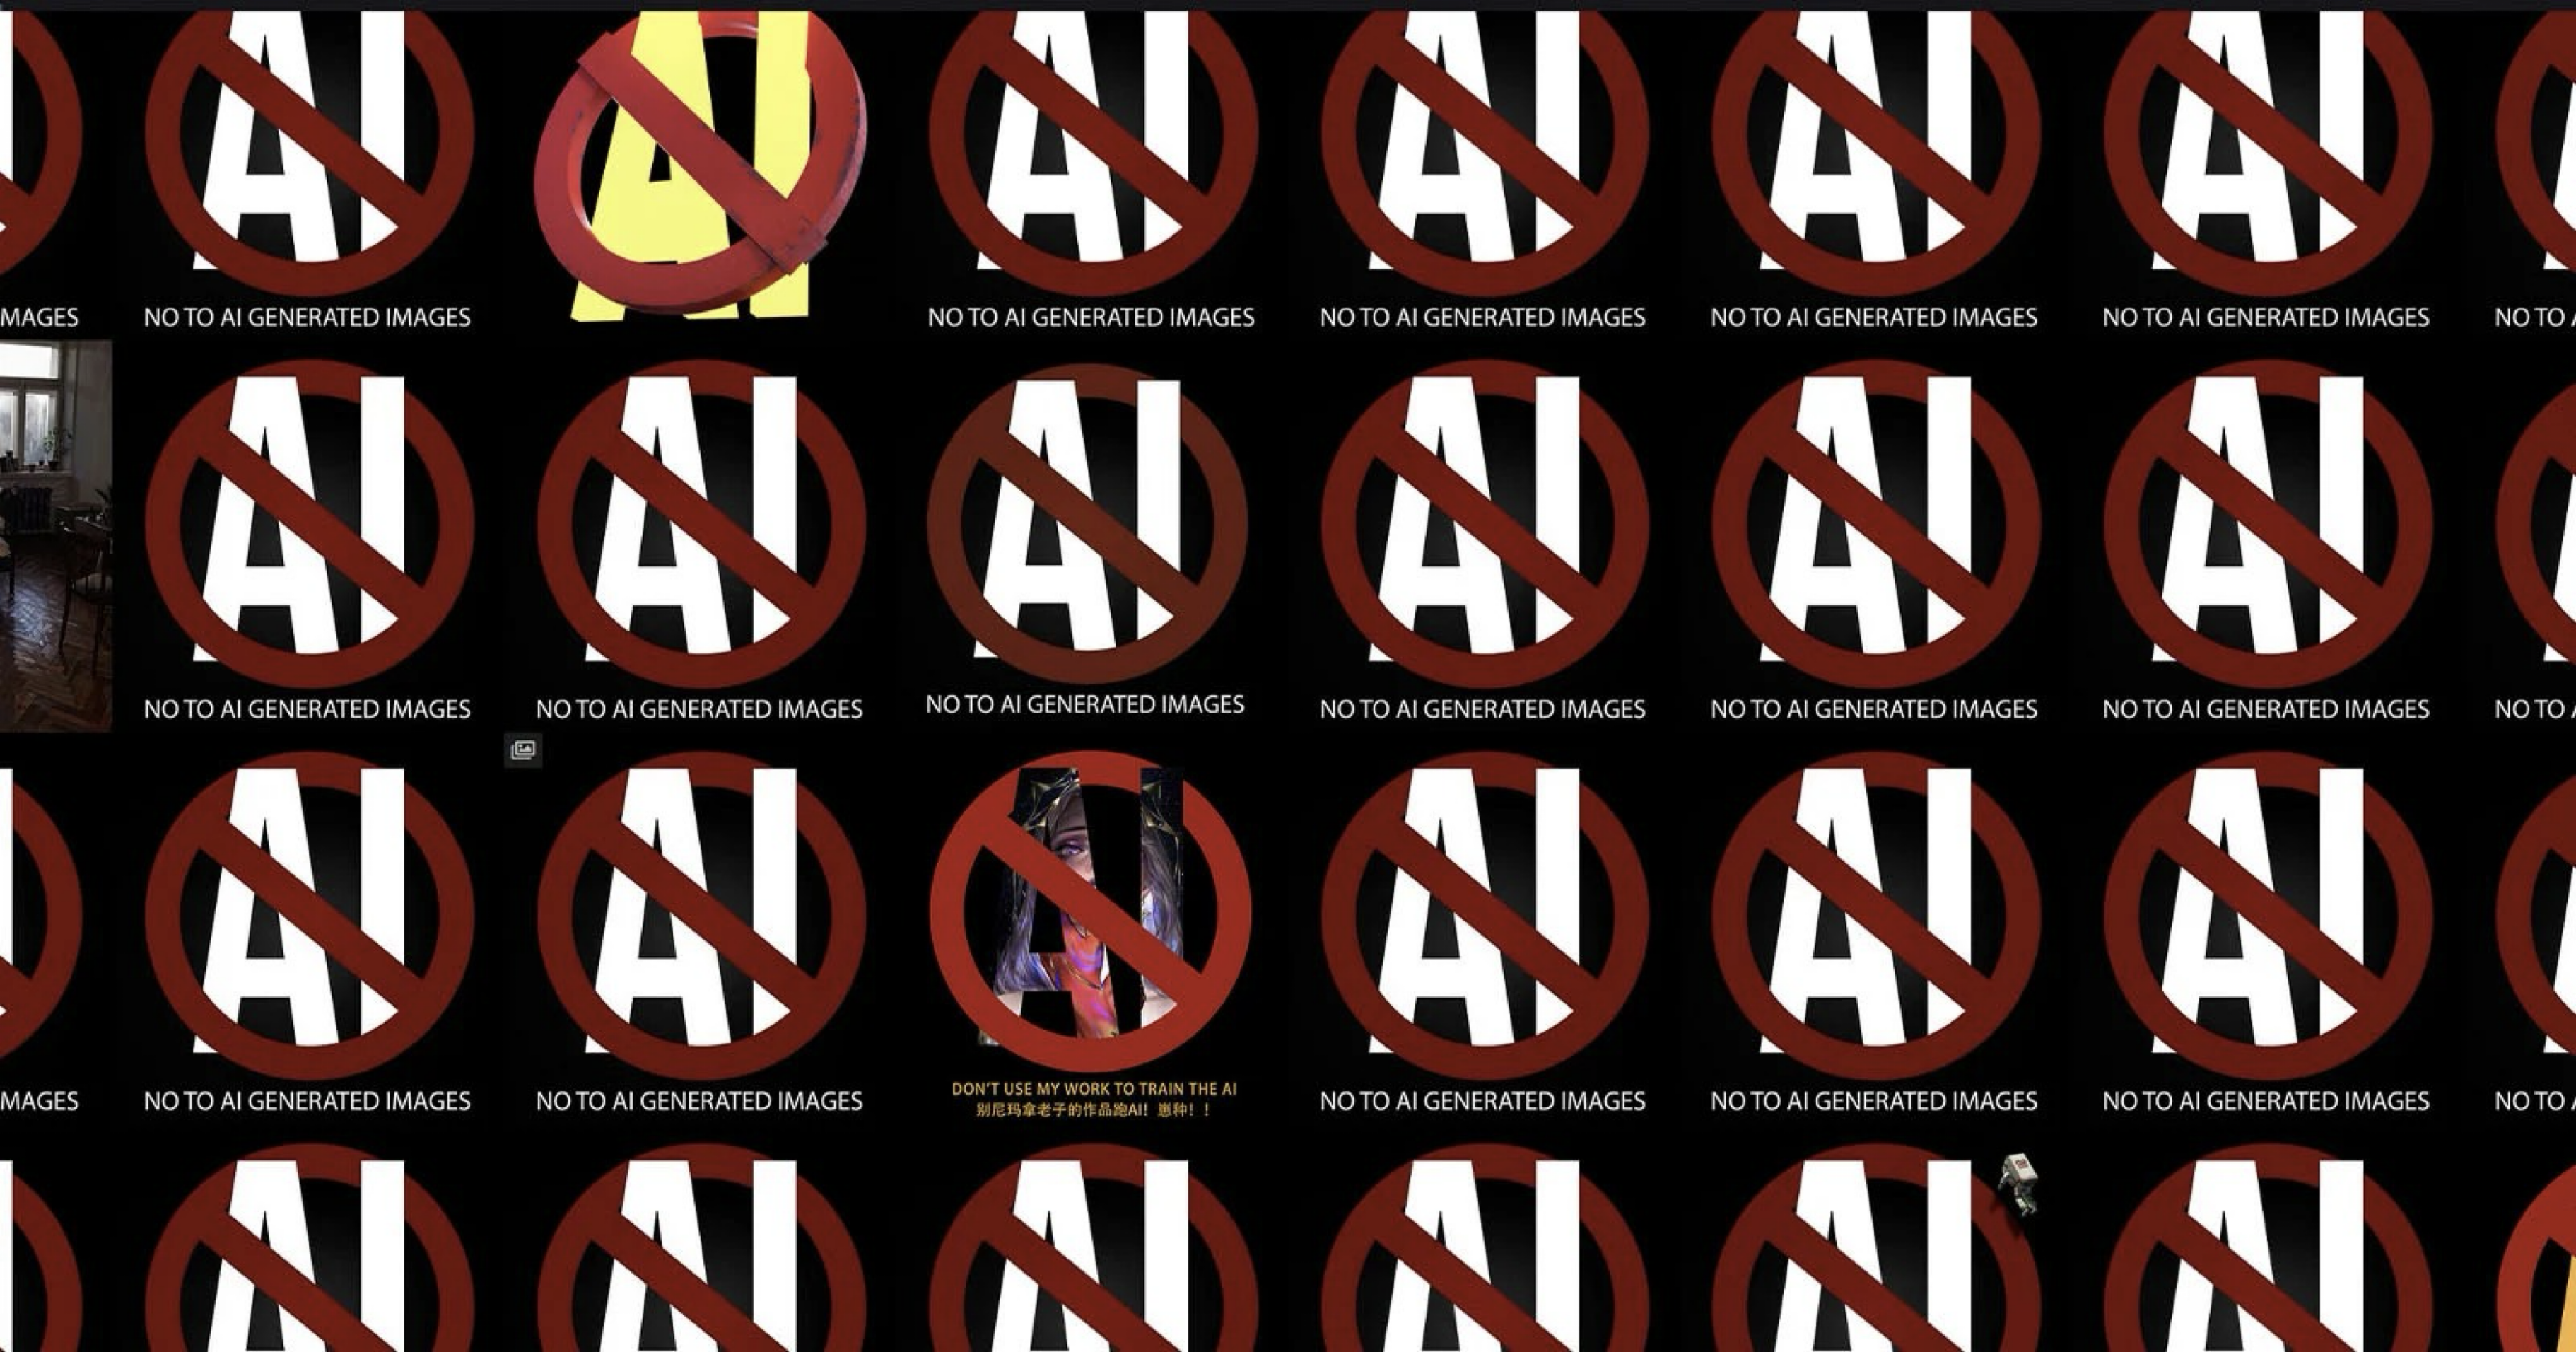
\includegraphics[width=1\textwidth]{figures/c1_intro/no-ai-art.png}
    \caption['No-AI memes being shared on the platform ArtStation]{Screenshot from the art platform \textit{ArtStation}, where memes with the caption `no to AI generated images' were shared widely in a large backlash to generative AI from traditional creative communities.}
    \label{fig:c1:no-ai-art}
\end{figure}

The outrage was levelled at developments in text-to-image models from startups such as \cite{midjourney2023midjourney} and \cite{stability2023stability}, that had been trained on large swathes of data collected from internet, including web platforms designed for people to share their art, as a means of having an online portfolio to raise their public profile, and in many cases, marketing their work for people to buy or to attract freelance work, or to gain employment as an artist, graphic designer, or illustrator.

While text-to-image models have been around for some time, the developments in 2022 with diffusion-based models such as \textit{Dall-E 2} \citep{openai2022dalle2}, \textit{MidJourney v4} \citep{edwards2022midjourney} and \textit{stable diffusion} \citep{stability2022stable}, and their ability to so successfully imitate the existing styles of individual artists, simply by listing the names of well-known creators on these digital platforms in the input text prompt, sparked outrage in the creative communities from which a lot of the data was sourced. 
A large part of the outrage was the use of the entire body of individual artists' works for training data without consent and without remuneration.
There are also legitimate and substantiated fears, that these generative AI systems will put creative practitioners out of work and lower the barrier to entry for image generation so considerably to make it a trivial pursuit requiring little skill or training to produce commercially viable results.
A recent statement, signed by tens of thousands of creative professionals and hundreds of creative industry organisations, expressed this sentiment in unequivocal terms:

\begin{quote}
`The unlicensed use of creative works for training generative AI is a major, unjust threat to the livelihoods of the people behind those works, and must not be permitted.' \citep{aistatement2024}
\end{quote}

% Much of the content shared in protest against AI-art was quoted with statements such as `AI is theft' \citep{whiddington2022backlash}, with trending hashtags like \#SupportHumanArtists \citep{zakuga2022theft}. 
% Several ongoing lawsuits have emerged against companies like MidJourney and Stability.AI, from artists themselves \citep{brittain2023artists} and from companies like Getty Images and Shutterstock that provide stock photographs and artworks \citep{vincent2023getty}. 
% Many artists have now removed their work portfolios from publicly available sites, and ArtStation and DeviantArt now have metadata tags for ‘NoAI’ \citep{artstation2022noai}, signalling that permission is withheld for those works to be used in creating datasets for training AI systems, which users on DeviantArt platforms are opted into by default \citep{deviantart2022optout}. 
% This trend of opting out of automated web scraping for AI training has been expanded to any website listed on the World Wide Web, with `ai.txt' files \citep{aitxt2024spawning}.
% Unsurprisingly, these meta-data tags are often ignored by web crawlers when scraping data for training generative AI models \citep{weatherbed2024anthropic}, and if these do not become legally enforceable at some point, it is predicted that online content producers will move away from the open-web and put their content behind paywalls \citep{longpre2024consent}.

Speaking as a researcher and practitioner in the direct field, it is my view the concerns and grievances of these artists are completely legitimate. 
I have been an active member of the CreativeAI community since its inception, and it is disheartening to see `big tech' startups entering this space and acting with such contempt for the communities of artists from which much of their value and power is sourced. 
The work in this thesis is positioned in opposition and as an alternative to the practices of these large tech organisations. 
The goal of this thesis has been to find new ways of \textit{making} with AI and find ways of creatively (mis)using these technologies in order to understand them better from the perspective of those in the arts \citep{salvaggio2023aarg}.
Throughout the development of this PhD research, I have sought to explore how we can create using generative AI without imitating data, and in addition, how we can use generative AI to create new styles and sounds without rehashing what humans have already created, and further, how we can learn more about how generative AI works by trying to interfere with its intended operation (\S \ref{ch:net_bend}; \S \ref{c8:sec:explaining}).

\section{Intellectual Property and AI Art}

My first encounters with the issues of copyright, ownership and authorship of work with generative AI predate these developments. 
In 2015-16, I was working towards a research Master's thesis in Creative Computing at Goldsmiths, University of London, just as generative AI research was beginning to demonstrate significant improvement in realism. 
In one of the experiments outlined in the thesis, I used all the frames from the film \textit{Blade Runner} as the training data for an autoencoder model, which after training I used to make a reconstruction of the film through the learned model \citep{broad2016autoencoding}  (Fig. \ref{fig:c1:blade-runner}).
The film \textit{Blade Runner -- Autoencoded} garnered a large international interest and I was very lucky to have had the work exhibited around the world in major museums and galleries \citep{broad2017autoencoding}  (Fig. \ref{fig:c1:blade-runner-whitney}).

\begin{figure}[!htb]
    \centering
    \captionsetup{justification=centering}
    \includegraphics[width=1\textwidth]{figures/c1_intro/blade_runner_still.png}
    \caption{Still from \textit{Blade Runner --- Autoencoded}.}
    \label{fig:c1:blade-runner}
\end{figure}

The training data, of course, was not intellectual property that I had permission to use.\footnote{It should also be noted that I was not even the first person to recreate \textit{Blade Runner} with machine learning. Ben Bogart's work \textit{Watching (Blade Runner)} was also created in 2016 \citep{bogart2016watching} (and built upon earlier research \citep{bogart2008memory,bogart2013context}), which I only learnt of its existence many months after completing my own recreation of the film.}
Ironically, this project and the resulting (and later rescinded) DMCA copyright takedown notice given to the videos on the web platform Vimeo was what catapulted the work to international recognition after an account of these travails was detailed in the news website Vox \citep{romano2016bladerunner}.

\begin{figure}[!htb]
    \centering
    \captionsetup{justification=centering}
    \includegraphics[width=1\textwidth]{figures/c1_intro/whitney-installation-shot.png}
    \caption[Installation shot of \textit{Blade Runner --- Autoencoded}]{Installation view of \textit{Dreamlands: Immersive Cinema and Art, 1905-2016} (Whitney Museum of American Art, New York, October 28, 2016-February 5, 2017). Left to right: Terence Broad, \textit{Blade Runner - Autoencoded}, 2016; Liam Gillick, \textit{Annlee You Proposes}, 2001. Photograph by Ron Amstutz. Image courtesy of the Whitney Museum of American Art.}
    \label{fig:c1:blade-runner-whitney}
\end{figure}

Though I did not face any further legal action from Warner Brothers for  disseminating the work, it was a major cause of personal stress, as I was very often anticipating some form of legal intervention (e.g. a cease and desist notice) from Warner Brothers prior to any exhibition where the work was going to be shown.
An opinion published in the Columbia Journal of Law and the Arts predicted that the work would probably be dealt with as copyright infringement were it tested in an American court \citep{sobel2017artificial}.\footnote{An alternative legal opinion was given by legal scholar Andres Guadamuz, who believed that this would would be protected by fair-use or fair-dealing if it were to be tested in court on the basis of parody or pastiche \citep{guadamuz2024personal}.} 
I produced the work before the widespread emergence of NFTs and before there was a large market for AI-generated artworks. 
The money I made from exhibition fees and selling editions of the video work would have been relatively insignificant for a multinational media company. 
Nonetheless, this experience was instrumental in informing the subsequent research presented in this thesis. 
Finding ways of using generative AI that does not rely on data and the intellectual property of others was a key aim for the research presented in this thesis.


\section{Motivation}

My goal was to find ways of training or configuring generative AI models which did not rely on the creation of datasets to produce creative outcomes. 
From working in industry, I had experienced how labour-intensive and time-consuming creating high-quality datasets could be, and it was clear this was a hugely time-consuming aspect of Generative AI research processes.
The second was to find ways of achieving novel outcomes that did not rely on access to high-end resources, for example, those available to large technology companies, including Google DeepMind, NVIDIA, or artists such as Refik Anadol (who reportedly have access to considerable computational resources  \citep{caulfield2022refik}). 
To this end, this research has focussed on exploring methods for training, configuring and customising very high-fidelity models that, when trained conventionally, require supercomputer-level resources. 
As such, this thesis presents a number of useful methods for manipulating, training and controlling these same models in much shorter time periods on consumer-level hardware.

Instead of relying on laboriously or ethically questionable datasets to try and achieve creative outcomes, the work in this thesis details data-free methods that push the possibility space of what can be generated with contemporary neural networks.
The approaches detailed are an attempt to use the intrinsic affordances of these neural networks to create original outputs that would not have been possible using any other technique or technology. 
The work detailed in this thesis is experimental image-making in its truest sense, and I have taken more inspiration from experimental photographers and filmmakers of the 20th Century (such as Harold Edgerton, Hiroshi Sugimoto, and Oskar Fischinger) than from academic researchers.

The driving force that led to each technical breakthrough in this thesis has been technical curiosity. 
When considering a new possible configuration for training an AI or some other kind of intervention, if I couldn’t imagine what the result of that experiment would look like, I would have to build it to find out, regardless of how many weeks or months of work it would take to get there. 
The results presented here are the experiments that produced the most surprising and striking results - sometimes beautiful and sometimes horrifying. 
There were a lot of failed experiments along the way that produced boring, predictable and uninspiring results. 
I’ve spared the reader details of most of these, apart from the few that led to key insights.

\section{Research Methods}

The research breakthroughs presented in this thesis have all come from a technological exploration of what is possible with these new technologies. Much of this research has been conducted in the vein of hacking, in its original meaning from the hacker culture at MIT in the 60s and 70s, where hacking meant `exploring the limits of what is possible, in a spirit of playful cleverness' \citep{stallman2002hacking}. 
This hacking ethos is not an approach that many people were taking in machine learning research when I started this PhD. 
The field was, and still is, very much dominated by orthodoxies and ideology, where theoretical mathematical underpinnings, achieving state-of-the-art performance on some widely used benchmark, and generalisation are most valued by the research communities \citep{birhane2022values}.

\textit{Hacking} was the primary means by which the algorithms in this thesis were discovered, but artistic exploration has also been central to the experimental work described in this thesis. 
When I started this PhD, my plan was to conduct primarily technical research and continue with an artistic practice on the side, maybe using some of the techniques developed in my research. 
Instead, it was an artistic enquiry that led me to the technical breakthroughs in the PhD, not the other way around. 

In his paper \textit{`Art in the sciences of the artificial'}, Stanley argues that in the fields of AI research and artificial life, subjective evaluation is a key driving force of progress for many researchers and practitioners in the field. 
There is a tendency in these research fields to discourage the dissemination of these observations in academic writing and in wider public discourse, something that Stanley worries might `cut off some future discoverers from what could have been their inspirations' \citep{stanley2018art}. 
In this thesis, I have sought to share my subjective position at various times in the thesis, and how that informed the direction of the following research experiments (\S \ref{c8:sec:aesthetic} for a further reflection on this).

Being both guided by, and disseminating this kind of subjectivity is commonplace in research practices in many areas of the humanities, including research methods such as autoethnography \citep{reed1997auto}, or practice-based and practice-led research \citep{candy2006practice}. 

The goal of this research has been at its core, to advance the creative possibilities of these technologies. 
As a practising and internationally recognised visual artist, my subjective understanding of the visual potential and aesthetics of these systems, has been one of the central guiding instruments in this research. 
To give any other account of how this research was conducted would be a failure of academic integrity. 

The work  I have done that is described in this dissertation and the contributions made in this thesis were the outcomes of practice-led research. 
The artistic outcomes are not presented as contributions to be assessed as outcomes of the thesis as such, but the process and practice that went into making them are described in an honest account in this thesis. 
Descriptions of artworks that have been made by myself and others using the techniques that have been described in this thesis are detailed in Chapter \ref{ch:impact}.

\section{Overview and Contributions of the Thesis}

The thesis is entitled \textit{Expanding the Generative Space}. 
The through line of all of the research presented here has been to find ways of going beyond the imitation of training data as the sole method for training generative neural networks. 
Instead, I have been trying to expand the possibility space that generative AI can produce, and the methods described in this thesis are but a few of the ways that this is possible. 

\subsection{Background}

Chapter \ref{ch:background} provides a thorough review of relevant background literature and related research conducted prior to the work presented in this thesis.
This review encapsulated both the technical aspects of machine learning relevant to this thesis, and also its application in creative contexts, whilst also drawing on the broader history of AI methods such as evolutionary algorithms, and their applications for generative processes. 
This chapter also describes notable prior work in relation to attempts to achieve novel outcomes with generative neural networks.

\subsection{Training without Data}

Chapter \ref{ch:unstable_eq} documents the first peer-reviewed and published approach to training generative neural networks without data, one of the three categorical contributions to active divergence methods (\S \ref{survey:nodata}) presented in this thesis.
This work was first published in the paper \textit{`Searching for an (un)stable equilibrium'}: experiments in training generative models without data' at the NeurIPS 2019 Workshop on Machine Learning for Creativity and Design \citep{broad2019searching}.

\subsection{Divergent Fine-Tuning}

Chapter \ref{ch:divergent} documents the first peer-reviewed and published approach to divergent fine-tuning of generative AI models without relying on imitation-based learning.
Divergent fine-tuning is another categorical contribution to active divergence methods (\S \ref{survey:divergent}) presented in this thesis.
This work was first published in the paper \textit{`Amplifying the uncanny'} at the 8th Conference on Computation, Communication, Aesthetics \& X (xCoAx) \citep{broad2020amplifying}.


\subsection{Network Bending}

Chapter \ref{ch:net_bend}, presents the network bending framework and is the third categorical contribution to active divergence methods presented in this thesis (\S \ref{survey:bending}).
This work was first published in the paper \textit{`Network Bending: Expressive manipulation of deep generative models'} at the International Conference on Artificial Intelligence in Music, Sound, Art and Design (EvoMUSART) \citep{broad2020network}, and later extended in the paper \textit{`Network Bending: Expressive Manipulation of Generative Models in Multiple Domains'} for the journal Entropy \citep{broad2021network}.
Network bending has been widely reused and adopted by many other artists and researchers (detailed in \S \ref{c7:sec:net-bend-artworks} \& \S \ref{c7:sec:net-bend-impact}).

\subsection{Active Divergence Taxonomy}

The final contribution of this thesis is the survey and formal taxonomy. 
The large majority of experimental work in this thesis falls under the umbrella term \textit{active divergence}. 
This was first coined by a PhD colleague and friend, Sebastian Berns and his supervisor Simon Colton [\citeyear{berns2020bridging}]. 
The core experimental work in this thesis pre-dates this definition, and I am indebted to Sebastian for summarising the overarching theme of my research, which felt far more disparate when I was working on it until he was able to summarise it in a two-word definition. 
In collaboration with Sebastian and Simon, I expanded on this definition and the paper \textit{`Active Divergence with Generative Deep Learning - A Survey and Taxonomy'} at the International Conference of Computational Creativity in 2021 \citep{broad2021active}.
An updated summary of that survey is presented in Chapter \ref{ch:active_div} and details work completed concurrently by others during the time of this PhD to achieve similar goals.

\subsection{Impact and Discussion}

Chapter \ref{ch:impact} details the impact of the research presented in this thesis and the subsequent work that this thesis went on to inspire. Chapter \ref{ch:discussion} reflects on the work undertaken, how artistic approaches to hacking AI models and training can lead to new forms of understanding, and how AI itself can be used as a material for artistic exploration and expression, a topic that I discussed in the paper \textit{`Using Generative AI as an Artistic Material: A Hacker's Guide'} that I presented at the 2nd international workshop on eXplainable AI for the Arts (XAIxArts) at the ACM Creativity and Cognition Conference \citep{broad2024using}.

\subsection{Conclusion}

Chapter \ref{ch:conclusion} concludes the thesis and reflects further on its contributions.
This chapter also details the limitations of the research presented in this thesis and discusses possible future research directions to take this work further.

\section{Summary}

In the six years that I have been working on this PhD, there has been a huge amount of upheaval in the research field and its impacts on wider society. 
I have seen AI art and generative AI go from a small, quirky community of enthusiasts to a booming industry that has become pitted against the interests and livelihoods of the creative professionals that they are extracting value from.
Hopefully, the approaches to working with AI described in this thesis can help others to find ways of using and working with generative AI which does not rely on the mass stealing and exploitation of creative professionals, but instead fosters new ways for creative people to use generative AI in ways that creative people will always do: to deliberately break, misuse and adapt technologies far beyond the intended purpose to forge new forms of creative expression.


\chapter{Background}
\label{ch:background}

\section{Introduction}

This chapter gives a background on the literature that was (mostly) available before I undertook my experimental research in 2018~19. 
The majority of this chapter outlines the technical basics of machine learning, neural networks and generative modelling. 
However, this is not the whole story. Many areas of research into computation, creativity, generative systems and divergent thinking existed before the advent of deep learning circa 2011. 

\section{Computation \& Creativity}

Since automated computing machines became a possibility, and the idea of writing programs in order to give these machines arbitrary instructions to follow, the idea of using computers to develop artefacts deemed creative has been long imagined. 
Ada Lovelace, the woman considered to be the first ever computer programmer, imagined that programmes for Charles Babbage's unfinished Analytical Engine could ‘compose elaborate and scientific pieces of music of any degree of complexity or extent’.
Lovelace however, did not think that computers could originate creativity themselves, declaring ‘The Analytical Engine has no pretensions whatever to originate anything. I can do [only] whatever we know how to order it to perform.' \citep{lovelace1843notes}.

Alan Turing took an opposing viewpoint to Lovelace on this question, stating that this objection would be better posed as ‘a machine can never ‘take us by surprise’’, countering that ‘Machines take me by surprise with great frequency [...] because I do not do sufficient calculation to decide what to expect them to do.’  \citep{machinery1950computing}
This reframing from originality to surprise moves to judgment shift from an action by the machine to an evaluation based on human reaction. 
Turing develops this further, by describing a scenario called \textit{The Imitation Game}, where a computer would be evaluated through a text channel and asked questions by an evaluator to differentiate whether it was human or not. 
If it succeeded in this challenge, this would be a threshold for determining intelligence,
this means of evaluating computational intelligence is commonly referred to as the Turing Test. 

In his description of the imitation game, Turing took seriously the idea of a computer being able to develop creative work. 
In the paper 'Computing Machinery and Intelligence' he muses about a machine writing a sonnet, and then, through the viva voce style of examination, be able to critically defend the work against a human interrogator based on criteria of aesthetic value, originality and of potential subjective readings of proposed changes to the language used in the work.

The idea that the bar for computational intelligence is to be able to convincingly imitate human behaviours, is one that has long been anchored towards. 
Imitation is central to much of how we train machine learning, neural networks and generative models. 
Though imitation alone does not have its controversies in being used as a benchmark for intelligence. 
An alternative theoretical test for computational intelligence is the Lovelace test, where a computational program would pass the test if it comes up with an original artefact (poem, musical score, novel, idea) that can be reproduced and that the creators of the program can not come up with an explanation for how the programme has found that solution \citep{bringsjord2003creativity}. 

\cite{ward2020computational} argues that Turing's characterisation of Lovelace's lack of faith in the possibility for the analytical engine to produce origination (that he equates with surprise) is a mischaracterisation and misunderstanding of the debates around mechanisation and origination that were happening during the industrial revolution. 
In the same notes where she makes her famous objection, she also goes on to say that the analytical engine has the power to offer new perspectives by combining theories in new ways \citep{lovelace1843notes}.
 Lovelace's remarks demonstrate the creative value of human-machine interaction, where she ``understand mechanicity not as inherently creative or uncreative but as a mode through which new kinds of creativity are possible'' \citep{ward2020computational}.

\subsection{Theories of Creative Processes}

Creativity itself is broadly agreed as a well-defined concept, though there are some differences in their definitions. 
Narrower definitions of creativity refer to the cognitive processes involved in culturally understood creative activities, such as 'pieces of music, sculpture, painting, poems or other things that are taken or presented as art' \citep{wiggins2015evolutionary}.
Creativity though, is used much more broadly in common language. 
It can also be applied to acts, ideas or behaviours outside of the realm of art-making, such as scientific fields, sports, economic activities or even mundane, day-to-day activities.


A broader definition of creativity is that it is an act that produces something \textbf{new and original} \citep{kaufman2021overview}. This act needs to be task-appropriate, fulfilling the requirements of whatever the original task set out. 
However, theories of how creativity is achieved, what facilities it, and how it is recognised and evaluated are far more disparate and less agreed upon. 

Theories of what makes a person creative, tend to focus on a summation of different elements. 
The componential model of creativity proposes that three interconnected variables are key to individual creativity.
Firstly there are domain-relevant skills and knowledge, such as a technical skill or specific talent.
Secondly, there are skills relevant for creative processes, such as a tolerance to ambiguity and a willingness to take certain risks.
Finally, intrinsic motivation is needed to take part in an activity because it is enjoyable and meaningful \citep{amabile1983social}.

There are many other theories of creativity, pertaining to evaluating individual persons' creativity, creative collaborations, understanding traits of creative peoples and situations that best facilitate creativity and how creativity is evaluated from a historical or cultural perspective. 
The outline in the rest of this section will only cover theories or models of creative processes, which have been developed in order to understand how to enhance and replicate creative acts, and in some cases, so that they can be partially or fully automated with computation.

\subsubsection{Convergent and Divergent Thinking}

The psychologist J.P. Guildford set out a series of traits and cognitive processes specific to creative activity. Those are ideation fluency, ideation novelty, synthesising ability and redefining ability, sensitivity to problems and evaluating ability \citep{guilford1950creativity}. The fluency with ideas generated, the novelty of said ideas and the ability to then critically evaluate those ideas and pick the best one being some of the most important traits for creative people
\footnote{Notably, Guildford motivates this early research into the psychology of creativity because of the rise of \textit{thinking machines} (aka digital computers).
Imagining their eventual knock-on effect on the labour market and a future industrial revolution of intelligence being automated, Guildford muses that the only economic value left of human brains would be in the creative thinking they are capable of \citep{guilford1950creativity}. 
A viewpoint I am not unsympathetic to.}. 

Guildford later builds on this theory, expanding the thinking processes needed in creative thinking, in particular the processes that are required for the production of creative ideas.
He differentiates two kinds of productive thinking that are required for creativity, which are divergent and convergent thinking. 
Convergent thinking is the focusing of ideas down to a single correct answer. Whereas divergent thinking is the diametric opposite, which is the ability to generate new and different ideas. 
In the context of modelling creative acts, these two types of thinking are also called idea generation and idea evaluation \citep{guilford1957creative}.

Of these two modes of productive thinking, Guildford believes divergent thinking is the one that is more representative and unique to the creative process. He places factors of fluency, flexibility and originality of thinking to all be products of abilities in divergent thinking. 
Guildford's ideas about divergent thinking went on to inspire many other aspects of research, such as the Torrance test for creative thinking \citep{torrance1966torrance}.

\subsubsection{Associative Creativity}

Associative creativity is the theory that creative people or creative acts are made when connections are made between remote concepts or ideas \citep{mednick1962associative}. 
Koestler coined the term \textit{bisociation} to describe a cognitive process where two or more concepts are combined to create a new concept \citep{koestler1964act}.
This model of creativity is also referred to as \textit{combinatorial creativity} \citep{boden2004creative}.

\subsubsection{Evolutionary Theory of Creativity}

Evolutionary theory states that the genetic structure of living beings is constantly changing through processes of random mutation and selection. Selection is carried out in two ways: \textbf{natural selection} is the process of fitness through living beings surviving long enough to reproduce sexually and transmit their genome, \textbf{sexual selection} is the process by which animals make preferential choices with what animals to mate based on particular attributes.

An evolutionary approach to how ideas are generated and selected in creative acts was proposed by \cite{campbell1960blind}, where he stated that the process of blind variation and selective retention in thought achieves innovation (aka creativity) through a process of internal emitting of thoughts, a process which lacks prescience and foresight. 
Campbell justifies this as a blind process as `once the process has blindly stumbled into a thought trail that ``fits'' the section criterion, accompanied by the ``something clicked' or ``Eureka'' that usually marks the successful termination of the process' \citep{campbell1960blind}.

\subsection{Computational Creativity}

Computational creativity is a subfield of artificial intelligence research, which investigates developing software that exhibits creative behaviours that unbiased observers would perceive as being creative \citep{colton2012computational}.
Computational creativity research is usually preoccupied with artefact generation, in domains that are culturally recognised as being creative, such as generation poetry, story generation, images or music. 
The quality of the generative processes themselves though is usually a secondary concern. 
The mechanics of the system and how they are constructed to imitate the creative faculties of humans are of more concern. 
Computational creativity differentiates itself from the practice of building creativity support tools that are commonly researched in human-computer interaction (\S \ref{c2:subsec:cst}).
Famously, the tagline at the 3rd International Conference on Computational Creativity in 2012 was ‘scoffing at mere creativity for more than a decade’, though this has an increasingly divisive phrase within the computational creativity community \citep{ventura2016mere}.

\subsubsection{Human-AI Co-Creation}

Human-AI co-creation (also referred to as co-cretivity), is a subfield of computational creativity research where the creative responsibility is shared between the software and the human interacting with it \citep{candy2002modeling}.
This framing puts the software as a creative collaborator, as opposed to an independent creative agent or tool only for supporting human creativity \citep{feldman2017co}.

\subsection{Metacreation}

A term related to computational creativity is \textit{metacreation}, which is a practice of developing software that demonstrates creative behaviour \citep{whitelaw2004metacreation}. 
In metacreation practice, the objective is not just to develop software, but to produce and present artistic works derived from the software, to validate their success. 
This is in contrast with computational creativity research, where the inherent soundness of the processes encoded in the system architecture is what determines their success \citep{colton2008creativity}.

\cite{eigenfeldt2012evaluating} describe five viewpoints that should be considered when evaluating a metacreation system: (1) the designer of the system, (2) the audience for the derived artworks, (3) academic experts, (4) domain experts, (5) results from controlled experiments.  

\subsection{Creative Computing}

Creative computing is an academic discipline\footnote{Creative computing is the academic discipline I am most at home with, having done my BSc and (integrated) Msci in Creative Computing at Goldsmiths, University of London, and more recently, being employed as a Senior Lecturer at the Creative Computing Insititute at University of the Arts London.}
that builds from the alternative computing scenes of the latter half of the 20th Century, which include  \textit{hacking} and \textit{the demoscene}. 
\textit{Hacking} and the creation of a \textit{hack}, is a specific sense of creative invention with given materials in the context of electrical engineering and the academic environments researching this in the 1960s in MIT and Stanford \citep{wark2006hackers}. 
Though not exclusively used to describe computer code or a technical system, a \textit{hack} had to ``be imbued with innovation, style and technical virtuosity'' \citep{levy1984hackers}.

Hacking later became associated with the breaking of digital security and performing acts of digital trespassing and accessing confidential information, a practice that has retrospectively been called cracking. 
Cracking copy protection on home computer systems, for the distribution of games led to the evolution of the \textit{demoscene}. In the demoscene,  visual and audio programs were written and freely shared, where value was determined by ‘more graphical elements, more mathematical effects and more sounds made a better demo, while bugs, glitches, and irregularities made the demo worse’ \citep{carlsson2019forgotten}.

Creative computing refers to the practice of using computing technologies to create expressive artefacts rather than something functional \citep{yang2016promoting}.
In creative computing, programming is the main tool that the creator uses to generate an artefact, and coding is the medium used to express human creativity. 

Creative coding is often carried out with creative coding frameworks, which are libraries, programming languages, or visual programming interfaces (such as node-based programming). 
Creative coding frameworks tend to focus on supporting visual rendering, audio processing and supporting human interaction with these frameworks. 


\subsection{Creativity Support Tools}
\label{c2:subsec:cst}

Creativity support tool (CST) is the term given to software programmes that are designed to facilitate creative acts or enhance a user's creativity \citep{shneiderman2002creativity}. 
For CST’s the graphical user interface (GUI) is of high importance \citep{shneiderman1999user}. 
CST’s can be used to facilitate many varieties of tasks such as searching, visualising, consulting, thinking, exploring, composing, reviewing and disseminating \citep{shneiderman2002cst_tutorial}.

With creativity support tools, the code is neither seen as acting in a creative way in its own right nor is it a medium for humans to be creative. 
Creativity support tools are independent pieces of software that can facilitate creativity but are not seen as being responsible for any part of the creative in their own right.

\subsection{Computational Models of Creative Processes}

There is a large existing literature of computational models, that encode specific theories of creative processes, or specific attributes that are deemed essential for creative people to have. 
This subsection covers a non-exhaustive selection of these methods described in the literature.

\subsubsection{Evolutionary Computation}

Evolutionary computation refers to algorithms that are inspired by the process of biological evolution to perform some form of optimisation. 
The most commonly used evolutionary algorithm is the \textit{genetic algorithm}, which is inspired by many of the processes present in biological evolution, such as random mutation, sexual selection, or (chromosomal) crossover.

Genetic algorithms require some kind of \textit{fitness function}, that determines the quality or performance of an individual solution to whatever optimisation problem is trying to be solved. This is analogous to the \textit{loss functions} used in machine learning algorithms (\S \ref{c2:sec:ml}). 

A genetic algorithm requires a genetic representation of the solution domain. 
This representation is usually a linear vector, and is often binary, with a fixed length representation, which allows for easy implementation of genetic operations such as crossover. 
The parameters in the genetic representation need to be carefully selected as they determine the \textit{solution space}.
Genetics algorithms are a stochastic optimisation process for exploring a \textit{fitness landscape} and converging onto a high-quality solution. 

% Human-based genetic algorithms replace the fitness function with a human evaluator

\subsubsection{Novelty Search}

Novelty search is an algorithm developed by \cite{lehman2008exploiting}, first used to guide evolutionary algorithms, where there is no set objective or fitness function, but instead, the search for novelty in the behavioural space of an evolutionary agent is the sole criteria. \cite{lehman2010efficiently, lehman2011novelty, lehman2011abandoning} argue that by abandoning prescriptively defined objectives, novelty search algorithms can better search the possibility space of an evolutionary landscape, and they show that this approach can lead to both unexpected and more optimal behaviours in evolutionary agents This approach to open-ended learning in evolutionary algorithms has inspired more recent developments in the space of open-ended reinforcement learning \citep{wang2020enhanced} (see \S \ref{c2:subsec:reinforcement} for a definition of reinforcement learning).

\subsubsection{Bayesian Surprise}

Bayesian Surprise \citep{itti2005bayesian,itti2009bayesian} is an algorithm that takes information from information theory and Bayesian statistics. 
They develop a mathematical formulation of surprise, that can be calculated with computational processing.
\cite{itti2005bayesian,itti2009bayesian} show that this computational measure closely correlates with human attention, through the measurement of gaze shift of human participants watching television broadcasts.

\subsubsection{Intrinsic Motivation}

In agent-based AI modelling, intrinsic motivation is defined as goals or objectives for the agent that are not determined by external stimuli or reward functions (aka external motivation), but by the internal state of the agent itself. 
Intrinsic motivation can be applied in reinforcement learning agents \citep{chentanez2004intrinsically} (\S \ref{c2:subsec:reinforcement}), and is motivated that not all objectives are universally useful \citep{barto2013intrinsic}.
Intrinsic motivation in AI is grounded in evolutionary theory \citep{singh2010intrinsically}, where an otherwise single mathematical function that defines a universal fitness function does not account for all behaviours and evolutionary strategies exhibited in real-world biological evolution.

\subsubsection{Compression Progress}

Compression progress \citep{schmidhuber2008driven} is a theoretical approach to training agents that relates to novelty search \citep{lehman2008exploiting} and intrinsic motivation in RL agents \citep{chentanez2004intrinsically}.
Schmidhuber defines compression progress as an agent that is constantly trying to efficiently represent prior actions in an environment and constantly seeking out new experiences that would satisfy a `intrinsic curiosity reward', which would drive the agent toward seeking out novel and unpredictable experiences.
Schmidhuber argues that this framework could be used for mathematical discovery, as well as art-making through `subjective beauty'.

\subsubsection{Combinatorial Creativity}

Combinatorial creativity is the description of a creative process where two or more concepts are combined together to make new ones \citep{boden2004creative}. 
This concept is essentially a rehashing of the concept of bisociation first proposed by \cite{koestler1964act}. 
Combinatorial creativity has been explored extensively in the context of computational creativity research \citep{zarraonandia2017using, guzdial2018combinets, guzdial2018combinatorial} and in explaining the psychology of scientific discovery \citep{simonton2021scientific, simonton2022serendipity}.

\subsection{Enacting Creative Processes in the Computational Arts}

Many artists have explored models of creativity and creative processes, through practice-based enquiry. 
Artists have made substantial contributions to this field and our understanding of non-human creativity, and the interactions between people and computers in exploring new possibilities for creative autonomy and creative collaboration.
A selection of these efforts is detailed in the following.

\subsubsection{Human-AI Co-Creation}

Harold Cohen, the pioneering computational artist. developed and worked with the AARON program and robotic painter (using an x-y plotter), to co-create paintings between 1972-2010 \citep{cohen2016harold}. 
The programme underlying AARON was developed by Cohen himself \citep{cohen1995further}, using deterministic software that was in a constant process of development. 
AARON has been described as a form of meta-art (or metacreation) \citep{mccorduck1991aaron}, where the artwork itself is the creation of a process that creates art.

The artist Sougwen Chung extends Cohen's work to create a practice that is centred around performative works where Sougwen collaboratively and interactively \citep{benediktsson2019human}.
Sougwen uses this practice to explore themes of increasing automation and co-existence between humans, algorithms and machines \citep{voss2021conversation}.

\subsubsection{Evolutionary Arts}

Many artists have explored the biological theory of evolution and evolutionary computation for artistic experimentation.
Karl Sims seminal experiments, explored evolutionary computation for the creation of computer graphics \citep{sims1991artificial} and 3D morphology and behaviours in artificial creatures \citep{sims1994evolving, sims2023evolving}.

The artist William Latham, alongside collaborator Stephen Todd, developed the FormGrow to evolve 3D computer models resembling organic life \citep{latham1992evolutionary}, with the aesthetic preference of the artist guiding the evolutionary process \citep{lambert2013emergence}.
Using aesthetic preferences to guide evolutionary systems was also utilised in the work Cellular Forms by \citep{lomas2014cellular}, to interactively explore the possibility space of simulations of growing cellular organisms.

\section{Machine Learning}
\label{c2:sec:ml}
Machine learning algorithms are algorithms that automatically improve from training data or experience. 
Given training data, a machine learning algorithm will build a model to make predictions or decisions without explicitly being told what decisions to make. 
Most machine learning algorithms use some form of optimisation and are optimised to minimise a loss function that is generally predetermined and task-specific. 
The process of optimising a machine learning model is referred to as \emph{training}. 
When training a machine learning model, the loss function on the training data will be minimised with the goal of maximising the accuracy for the specific task. 
The model is generally evaluated on a separate test dataset that contains data not used during the training phase. 

\subsection{Supervised Learning}

Supervised learning algorithms build models based on training data that contain the desired set of output and inputs. 
This type of training data is referred to as \emph{labelled data}. 
A labelled dataset will consist of pairs of data, where every input will be given with a corresponding output. 
Labelled datasets are in most cases, hand-labelled by human users who ideally have expertise in the subject domain. 
Three of the most common tasks in supervised learning are \emph{classification}, \emph{regression} and \emph{metric learning}. 

In classification, each data sample $x$ will be paired with a vector $c$ that represents the class label. 
The machine learning model will take $x$ as an input and output a prediction $c'$. 
The objective during training is to maximise that the probability of the prediction $c'$ will match the value of the true label $c$. 

In regression, each data sample $x$ will be accompanied by an output $u$, where the output values are numerical values within a given range. 
The model will learn to output predictions $p'$ for input $x$. The goal of training a regression model is to learn a model that can generalise to unseen data, where the input and output values are not necessarily present in the training data but can be inferred based on the examples given in the training data. 

The goal of metric learning is to learn a distance function between given samples, that can be used to estimate how similar or dissimilar samples are. 
The model learns to provide a distance function $d(x,y)$ for input examples $x$ and $y$. In the labelled dataset, input examples are usually accompanied by a vector label $c$ donating the identity of the input example. 
When training a model, the goal is usually to minimise the distance between samples that have the same identity but maximise the distance between samples that have separate identities.

\subsection{Unsupervised Learning}

Unsupervised learning algorithms find patterns in data where there are no given labels. 
Unsupervised learning methods find patterns and structures within data without guidance, either by learning discriminative features or capturing patterns as probability densities. 
The two most common tasks in unsupervised learning are \textit{clustering}, \textit{dimensionality reduction} and \textit{generative modelling}.

Clustering is the task of grouping data into clusters such that data grouped together in the same cluster are more similar to each other than data in another cluster. 
Examples of algorithms used for clustering are K-means, Gaussian mixture models or density-based clustering methods.

Dimensionality reduction is the task of transforming high-dimensional data into a lower-dimensional representation that still retains key characteristics present in the original data. 
Examples of algorithms used for dimensionality reduction are principle components analysis (PCA) t-distributed stochastic neighbour embedding (t-SNE) and autoencoders (see \S2.2.1). 

Generative modelling is the task of learning a function that can generate a given data distribution. 
A generative model will give a joint probability distribution between the observable and target variables. 
Approaches to generative modelling include Gaussian mixture models, hidden Markov models and neural networks. 
An overview of generative model approaches using deep neural networks is given in \S2.2.

\subsection{Reinforcement Learning}
\label{c2:subsec:reinforcement}

\section{Artificial Neural Networks}

Artificial neural networks are ensembles of connected units that are meant to loosely model the synaptic structure of biological neural networks. 
In 1958 Frank Rosenblatt built the Mark 1 Perceptron \citep{rosenblatt1958perceptron}, initially a physical circuit that was designed to perform the binary classification of images captured from a sensor array. 
The values of the weights between connections were encoded using potentiometers with a learning rule updated with electric motors. 
Later the perceptron architecture was modelled in software rather than hardware, with weight parameters and values encoded as real-valued numbers. 
The term perceptron was later used to donate a unit (or node) within a larger network and is used to this day in larger network architectures such as multi-layered perceptrons (MLP). 

The term multi-layered perceptron usually denotes a fully connected feed-forward neural network architecture with one or more hidden layers. 
However, MLP can also be used to refer to neural networks with more complex topological arrangements between nodes. 
MLPs can employ different non-linear activation functions, such as $\tanh$ and the sigmoid function ($\sigma$). 
A significant advance in training MLP networks came with the backpropagation algorithm \citep{werbos1974beyond}, where the gradient of the loss function is calculated and backpropagated through the network graph and used to adjust the weight parameters of the networks with respect to a single input pass of the network. 
This learning algorithm is referred to as gradient descent when the learning rule is applied after performing a forward pass on every datum in the dataset, and stochastic gradient descent (SGD) when it is applied after every sample or every batch of samples. 

\subsection{Deep Learning}

Deep learning is the term donated to the use of artificial neural networks with many hierarchical layers that produce \textit{deep} network structures. 
Earlier attempts to make neural network architectures with many layers were hampered by computational resources and limited availability and storage of data. 
The first major breakthrough in the efficacy of training deep generative models was to train a hierarchy of restricted Boltzmann machines \citep{ackley1985learning} as pretraining for a deep autoencoder network \citep{hinton2006reducing}. 
The first major breakthrough in efficacy and efficiency of training deep neural networks on graphics processing units (GPU) was with AlexNet \citep{krizhevsky2012imagenet} which won the 2011 ImageNet large-scale vision recognition challenge (LSVRC) for image classification \citep{russakovsky2015imagenet}. 
Additional breakthroughs in novel activation functions such as the rectified linear unit \citep{nair2010rectified}, and optimisation algorithms with improved performance and stability over SGD, such as RMSProp \citep{tieleman2012lecture} and ADAM \citep{kingma2015adam} were key to allowing for reliable training of large scale deep neural networks. 

\subsection{Neural Network Architectures}

Traditionally the most commonly used architecture for neural networks was the fully connected MLP, where every node in the layer of the network (perceptron) is connected to every other node in the previous and following layers. 
In more complex architectures, techniques like \textit{skip connections} are used to connect nodes from layers that have intermediate layers in between them. 

There is a range of other neural network architectures that have been found to have good performance for specific domains. 
Discussions of some of the most common ones are discussed in the following.

% (sparse networks? neuroevolution?)

\subsubsection{Convolutional Neural Networks}

A convolutional neural network (CNN) \citep{fukushima1982neocognitron} is a network that uses a structure of shared weights based on convolutional kernel filter functions, where the parameters of the convolutional kernel are learned. 
The kernel functions are repeated across the breadth of the input (in a sliding window fashion where the gap between each instance of the filter being applied is known as the \textit{stride}), ensuring that the learned features are equivariant to translation. 
CNN architectures are most commonly used in a 2-dimensional (2D) form for image processing, but 1D and 3D convolutional architectures are sometimes used for processing audio and 3D voxel data. 
In the architectures of generative models, transposed convolutions are commonly used to iteratively upsample learned features into a high-dimensional output.

\subsubsection{Recurrent Neural Networks}
\label{c2:subsubsec:rnn}

Recurrent neural networks (RNN) are neural network architectures that have connections between nodes along a temporal sequence. 
Connections from a previous temporal state into an existing state allow RNNs to exhibit dynamic temporal behaviour. RNNs are trained on sequential data, with activations from the previous state of the network feeding into the current state, and are able to process temporal data of variable lengths. 
Traditional RNNs suffer from the exploding and vanishing gradient problem, where the error signal backpropagated through the temporal state of the network has a tendency to vanish completely and prevent the network from learning or to explode and catastrophically lose information that had been acquired in training \cite{hochreiter1998vanishing}. 
RNN architectures such as the long-short term memory network (LSTM) \citep{hochreiter1997long} or the gated recurrent unit (GRU) \citep{cho2014properties} are specifically designed to avoid this problem by using gates that can retain information within the network for long periods of time and allow the network mix information from high frequency and low-frequency components. 

First introduced in the context of machine translation, the attention mechanism was introduced to improve the ability of RNNs to attend to different parts of the input and output sequences when predicting the next token \citep{bahdanau2014neural}. 
This attention mechanism has become widely used in many other domains and is now central to the functioning of large language models using the transformer architecture (\S \ref{c2:subsubsec:autoregressive}).

 
\section{Generative Neural Networks}

Generative models are neural networks that learn a set of neural network parameters that approximately model a target data distribution. 
This was generally seen as a difficult problem, especially for images and audio, until advances were made in techniques (listed below) and architectures were combined. 
Since 2015 there has been a lot of interest in generative models from varying research areas (computer graphics, audio digital-signal processing (DSP), human-computer interaction (HCI)) and creative communities, artists, musicians etc, because of their ability to produce artefacts of high cultural value. 

When training a generative model, a network architecture will be defined and the parameters of the network will be randomly initialised (see Figure \ref{fig:c2:gen-model-parameters}), the network will generate a sample $p'$ given an input vector $x$. 
Over the course of training using some learning rule, generated samples are optimised to resemble samples drawn from the target distribution $P$, eventually leading to a set of parameters that produces the approximate distribution $P'$.

All deep generative models, and in particular ones that generate high dimensional data domains like images, audio and natural language, will have some level of divergence $D(P||P') \geq 0$ between the target distribution $P$ and the approximate distribution $P'$, because of the complexity and stochasticity inherent in high dimensional data. 
The goal of all generative models is to minimise that level of divergence, by maximising the likelihood of generating the given data domain. 
Figure \ref{fig:c2:gen-model-distribution}, illustrates how after training the approximate distribution may be close to but not exactly the same as the target distribution, either by missing aspects from the original distribution or by containing elements not present in the true distribution. 

\subsection{Approaches to Modelling Data}

Approaches to modelling data distributions can be separated into three categories: explicitly - where modelling the likelihood of the data distribution is learned explicitly in the objective function, such as with autoencoders, autoregressive models and flow-based models; approximately - where an approximation of the target distribution is learned, as is the case with variational autoencoders (VAE); or implicitly - where the target data distribution is not modelled directly but is learned implicitly through an indirect training process as is the case with generative adversarial networks (GAN).
In the following subsection, more detail of the varying approaches to modelling data distributions is given. 

\subsubsection{Autoencoders}

An autoencoder is a symmetrical neural network that learns to reduce the dimensionality of a data domain. 
The first part of the network, the \textit{encoder} takes data from the input domain and compresses it into a latent representation $z \in Z \in \mathbb{R}$. 
The other half of the network is the \textit{decoder}, which takes the latent encoding that reconstructs the input. 
The encoder can be thought of as a learned algorithm for dimensionality reduction, and the decoder as the inverse function. 
Autoencoders are used for the tasks of dimensionality reduction, representation learning and generative modelling.

The variational autoencoder (VAE) \citep{kingma2013auto, rezende2014stochastic} advances the traditional autoencoder forces a distribution on the latent variable and uses Kullback-Liebler divergence (KLD) in the loss term to penalise the encoder from the posterior deviating too far from the prior distribution (usually a Gaussian). 
Using the reparamitsation trick, noise is injected into the latent space. 
As noise is injected into the latent space, a VAE models a data distribution approximately, in contrast with a traditional autoencoder which models a distribution explicitly and can only therefore model the lower bound of the log-likelihood of the data. 

\begin{equation}
\label{eq:vae}
L(x) = -D_{KL}(q_{\phi}(z|x)||p_{\theta}(z)) + E_{q_\phi}(z|x)(log_{p_{\theta}}(x|z))
\end{equation}

\subsubsection{Generative Adversarial Networks}

The generative adversarial network training framework (GAN) \cite{goodfellow2014generative} is a method of training generative models without directly approximating the target data distribution. 
Two networks, the generator and discriminator are set against each other in a zero-sum mini-max training regime. 
The discriminator is optimised to correctly classify real samples from a training set and fake samples from the generator, where the generator is optimised to fool the discriminator into thinking its samples are real, using the value function: 

\begin{equation}
\label{eq:gan}
\min_{G}\max_{D}\mathbb{E}_{x\sim p_{\text{data}}(x)}[\log{D(x)}] + \mathbb{E}_{z\sim p_{\text{z}}(z)}[1 - \log{D(G(z))}]
\end{equation}

\subsubsection{Auto-Regressive Modelling}
\label{c2:subsubsec:autoregressive}

An autoregressive generative model learns a conditional probability of a single output element based on the preceding elements. 
By using the chain rule, it is possible to backpropagate gradients through the network architecture \cite{larochelle2011neural}. 
Like RNNs, autoregressive models can be used to model sequential data of variable length, however, unlike RNNs the internal state of the network from previous time steps is not fed back into the state of the present time step. 
When generating from a trained autoregressive model, generated samples can be fed back into the model to generate novel continuous sequences.

The transformer architecture used foremostly in large language models (LLMs) \citep{vaswani2017attention}, makes use of the attention mechanism first introduced in RNNs \citep{bahdanau2014neural} (\S \ref{c2:subsubsec:rnn}), but removes the recurrent part of the model architecture.
In transformers, a fixed window of tokens (aka context length) is both given as input and output to the model.
In the generative context, the output to the model is offset from the input by a single token, and the model is trained to autoregressively predict the next token in the output based on the input, an approach most famously used by the GPT (generative pre-trained transformer) class of models \citep{radford2018improving, radford2019language,brown2020language}.

Autoregressive modelling has also been applied to image generation.
PixelCNN uses convolutional neural networks to generate images pixel-by-pixel using neighbouring pixels to determine what the next pixel should be \citep{van2016conditional}.
This can be used for both image in-painting, completion and unconditional image generation.
VQ-VAE (vector-quantised variational autoencoder) adapts the autoencoder approach so that the encoder produces discrete represenetations, and the decoder uses an autoregressive approach to sampling from these discrete codes, to improve the fidelity of generated images \citep{van2017neural}. 

\subsubsection{Reverse Diffusion Generative Models}
\label{c2:subsubsec:diffusion}

Reverse diffusion generative models take inspiration from thermodynamics, where they learn to reverse the process of diffusion applied to a particular data domain \citep{sohl2015deep} (such as images, audio or video). 
During training, noise is progressively added to data, to slowly destroy the structure in the data.
A neural network model, usually some adaption of a U-Net architecture \citep{ronneberger2015u} is trained to invert this diffusion process.
After training the model is able to unconditionally generate images from noise, by iteratively denoising them, as well as perform tasks like noise reduction and in-painting. 
The iterative approach to diffusion greatly enhances the fidelity and flexibility of generative models to model very diverse datasets.

\section{Analysis of Neural Networks} 

Developing methods for understanding the purpose of the internal features (aka hidden units) of deep neural networks has been an ongoing area of research. 
In computer vision and image processing applications, there have been a number of approaches, such as through visualisation, either by sampling patches that maximise the activation of hidden units \cite{zeiler2014visualizing, zhou2014object}, or by using variations of backpropagation to generate salient image features \cite{zeiler2014visualizing, simonyan2013deep}. 
The deepdream algorithm \citep{mordvintsev2015inceptionism} extends this approach but uses gradient-based optimisation to progressively alter images to maximise activations of certain hidden units, which gives the resemblance of psychedelic experiences \citep{suzuki2017deep}.
The artist Tom White, uses gradient-based optimisation to generate abstract images that resemble visual objects using image classifier networks in the series of artworks \textit{Perception Engines} \citep{white2018perception}.
By optimising towards an ensemble of classifier networks \cite{white2019shared} is able to show that there are shared visual representations between neural networks for image recognition and human visual representations.

\subsection{Analysis of Generative Neural Networks}

Understanding and manipulating the \emph{latent space} of generative models has subsequently been a growing area of research. 
Semantic latent manipulation consists of making informed alterations to the latent code that corresponds to the manipulation of different semantic properties present in the data. 
This can be done by operating directly on the latent codes \citep{brock2016neural, shen2020interpreting} or by analysing the activation space of latent codes to discover interpretable directions of manipulation in latent space \citep{harkonen2020ganspace}. 
Evolutionary methods have been applied to search and map the latent space \citep{bontrager2018deepmasterprints, fernandes2020evolutionary} and interactive evolutionary interfaces have also been built to operate on the latent codes \citep{Simon-ganbreeder} for human users to explore and generate samples from generative models. 

Network dissection \citep{Bau2018-td}, discussed in the previous subsection, was later adapted and applied to generative models \citep{Bau2018-td}, by removing individual units, while using in combination a bounding box detector trained on the ADE20K Scene dataset \citep{zhou2017scene}. 
This led to the ability to identify a number of units associated with the generating of certain aspects of the scene. 
This approach has since been adapted for music generation \citep{Brink2019-gc}. 

\section{Creative Practice with Generative Neural Networks}

Generative neural networks have become widely adopted in creative practice, through individual artistic practices, and in interactive applications and installation artworks. 
These are detailed in the following subsections.

\subsection{AI-Art} 

Artists have been experimenting with and creating artistic practices with AI in its various incarnations since the 1970's, with artists such as Harold Cohen, Peter Beyls, and Naoko Tosa making art with classical forms of AI techniques \citep{grba2022deep}. 
Since the advent of modern generative AI, using deep learning approaches to building and training neural networks, there have been many artists adopting these technologies in their creative practice from 2015 onwards (myself being one of them). 

Artists such as Helena Sarin, Anna Ridler, Gene Kogan, Mario Klingemann, Derrick Schultz, Tom White, Jake Elwes, Scott Eaton, and Sofia Crespo have all developed artistic practices centred around generative AI, often using these methods to create art around a particular social or environmental theme \citep{grba2022deep}. 
In many of these artistic practices, artists use generative models as artistic tools or as artistic materials (see Chapter \ref{ch:discussion} for a further discussion on this approach), which are playfully experimented with in order to craft unique forms of expression and artistic styles.
Many of these artists will create their own custom datasets that they use to train individual models or sets of models that are chained together in order to produce unique artistic styles (\S \ref{c2:subsec:divergent-practice}; \S \ref{survey:chaining}).

Many of these artists created work under the `CreativeAI' banner, a subcommunity of creative practitioners using early deep learning technologies like generative AI, as well as related techniques like deepdream and style transfer \citep{gatys2016neural} to make artworks. 
Lots of this work was on social media channels such as Twitter and Instagram, as well as in online digital art galleries such as the NeurIPS Creativity Workshop AI-Art Gallery\footnote{\url{https://www.aiartonline.com/}} and Computer Vision Art Galleries\footnote{\url{https://computervisionart.com/}}, primarily curated and organised by the curator Luba Elliot. 
Many of these artists also disseminated and sold artworks on blockchain-based NFT (non-fungible token) art platforms like \textit{hic et nunc}\footnote{\url{https://hicetnunc.art/}}, \textit{SuperRare}\footnote{\url{https://superrare.com/}}, \textit{Foundation}\footnote{\url{https://foundation.app/}}, and \textit{Feral File}\footnote{\url{https://feralfile.com/}}. 
It is now common for mainstream AI conferences to now have their own art galleries showcasing AI-art or CreativeAI tracks, such as the CVPR AI art gallery\footnote{\url{https://thecvf-art.com/}}, the SIGGRAPH\footnote{\url{https://s2024.siggraph.org/program/art-gallery/}} and SIGGRAPH Asia Art Galleries\footnote{\url{https://asia.siggraph.org/2024/submissions/art-gallery/}} or the NeurIPS CreativeAI track\footnote{\url{https://neurips.cc/Conferences/2023/CallForCreativeAI}}.

\subsection{Interacting with Generative Neural Networks} 

In this section, we detail a number of projects (interactive installations and creativity support tools) that allow for users to directly interact with generative neural networks.

\subsubsection{GAN Paint}

An~interactive interface built upon the GAN Dissection approach \citep{Bau2018-td} was presented with the GANPaint framework in 2019 \citep{bau2019semantic}. 
This allows users to `paint' onto an input image in order to edit and control the spatial formation of hand-picked features generated by the GAN. 

\subsubsection{GANBreeder}

GANBreeder (now rebranded as ArtBreeder) \citep{simon2020artbreeder} is a platform that allows users to collaboratively explore the latent space of a GANs.
GANBreeder was directly inspired by the PicBreeder experiment \citep{secretan2008picbreeder,secretan2011picbreeder} which was an online platform that allowed users to collaboratively explore the generative space of an early form of generative neural network, composition patter producing networks (CPPNs) \citep{stanley2007compositional}.
Both of these approaches provide a collaborative, interactive evolutionary approach to explore the generative space of neural networks. 
In PicBreeder this generative space is determined by the architecture of CPPNs, whereas in GANBreeder it was determined by the latent space of GANs.
In GANBreeder, users could interactively mutate, and cross-breed latent codes, creating new generative samples that are published on a shared collaborative platform.
The whole network of prior generations from the user and other users can be seen and interacted with.

\subsubsection{Learning to See}

\textit{Learning to see} is a series of artworks by the artist and researcher Memo Akten \citep{akten2019learning, celis2021memo}.
The artworks are presented as interactive installations.
In \textit{Learning to See: Hello, World!} the process of learning is performed in realtime, using the live camera feed of the user as the training dataset, training a VAE \citep{akten2017hello}.
In  \textit{Learning to See: Interactive}, pretrained image-to-image translation model (presumable CycleGAN, though the exact approach is not specified in \citep{akten2019learning}) are used in conjunction with a live webcam feed arranged at mundane objects (such cloth, cables, and car keys).
The image translation model takes the live feed of mundane objects and outputs a scene from whatever domain the image translation model was trained to output (such as oceans, flowers, and outer space) \citep{akten2017interactive}.

\subsubsection{Interactive Text Generation with RNN Ensembles}

\cite{akten2016real} presents a framework for real-time interactive text generation using an ensemble of recurrent neural networks. 
Here the outputs of many different models trained on different datasets (the Bible, the collected works of Aristotle, Jane Austen and Charles Baudelaire) are then interactive and fused together in a generative ensemble.
Here the probability of outputs for the next character are interpolated based on the specified mix by the user (this project is also detailed in \S \ref{survey:blending}).

\subsubsection{Text-to-Image Generation}

Text-to-image generation using generative neural networks was first presented by \cite{mansimov2015generating}.
They utilised the Deep Recurrent Autogressive Writer (DRAW) \citep{gregor2015draw}, which is a recurrent neural network that utilises attention layers for generating images in an autoregressive fashion.
\cite{mansimov2015generating} train this model on the MSCOCO dataset (Microsoft Common Objects in Context) \citep{lin2014microsoft}, which provides pairs of images with text captions, to condition a DRAW network on the captions.
After training, it is then possible to generate new images on image captions.

Conditioning the generation of an autoregressive generative model with an auxiliary network that can give a distance metric function for images and text was developed with the DALL-E model \citep{ramesh2021zero}.
Here they condition the training and generation of a VQ-VAE \citep{razavi2019generating} with CLIP (contrastive language-image pretraining) \citep{radford2021learning}.
Later approaches of text-to-image generation utilise CLIP conditioning for training and generation of diffusion and latent diffusion models (\S \ref{c2:subsubsec:diffusion}) for high fidelity text-to-image generation \citep{rombach2022high}.


\section{Data Divergent Generation with Generative Neural Networks}
\label{c2:sec:data-divergent}

This section details data-divergent generation with generative neural networks. 
This section is limited to methods that pre-date the research conducted in this thesis.
A full account of data-divergent generation with generative neural networks (aka active divergence) is given in Chapter \ref{ch:active_div}.

\subsection{Novelty Generation with Imitation Based Generative Modelling}

\citet{kazakcci2016digits} present an algorithm that performs novelty search over the learned generated samples of a sparse autoencoder trained on the MNIST dataset of handwritten digits \citep{lecun1998gradient}.
After training the autoencoder, they generate and map out the entire generative space, then use clustering algorithms to cluster the latent space into discrete clusters based on visual similarity, and then disregard clusters that map to existing labelled classes in the training dataset, leaving only clusters that map to new modalities of generation not present in the original training set (this approach is covered in more detail in the active divergence survey \S \ref{survey:noveltysearch}). 
\citep{cherti2017out} extend this approach to training a class-conditional generative model. 
They utilise hold-out classes, which automatically capture these modalities not present in the training set. 
Allowing for these novel modalities to be generated without the need for searching the latent space (this approach is covered in more detail in the active divergence survey \S \ref{survey:noveltygeneration}).   

\subsection{Creative Adversarial Networks}

In the Creative Adversarial Networks (CAN) framework, \cite{elgammal2017can} train a class-conditional generative model (using GAN-based adversarial training \citep{goodfellow2014generative}) on the wikiArt dataset \citep{saleh2016large}. 
The generator network is optimised to diverge from existing art styles and generate samples that sit within these existing art styles, to generate new `artworks' that have their own distinct styles that sit outside the art-historical framework.
This approach is inspired by Martinale's theory of artistic change \citep{martindale1990clockwork} where artists push against the habituation of existing artistic styles, yet still aim to minimise negative reactions from observers. 
The CAN framework is discussed further \S \ref{survey:noveltygeneration} in the discussion of its context in other approaches of active divergence. 

\subsection{CombiNets}

The CombiNets framework \citep{guzdial2018combinets} is inspired by combinatorial creativity  \citep{boden2004creative} where the learned parameters of multiple neural networks are combined together in order to create a new network with parameters from multiple networks.
This is done in a directed fashion where new samples outside of the training datasets of either of the existing models, for instance, a mythical creature like a pegasus, which combines characteristics of two real animals (horse and bird).

\subsection{Data Divergent Generation in Creative Practice}
\label{c2:subsec:divergent-practice}

One approach that many artists take using generative models, to diverge from existing training data, and create bespoke artistic styles is to chain multiple models together. 
This is commonly done by combining unconditional generative models (such as GANs or VAEs) with image-to-image translation models (such as Pix2Pix or CycleGAN) and other deep learning approaches such as style-transfer.
Artists like Helena Sarin use this to great effect to create unique artistic styles by combining many custom-trained generative models on their own hand-crafted datasets \citep{sarin2018playing}, deliberately utilising the imperfections of generative models to enhance their unique artistic style. 
This approach is detailed further in the active divergence survey as the `chaining models' approach \S \ref{survey:chaining}.

Another approach to data divergent generation comes from Mario Kinglemann in the project \textit{Neural glitch} \citep{klingemann2018neural}. 
Here Klingemann deliberately corrupts the learned weights of a generative model, by randomly deleting (zero-ing out) or swapping the learned parameters of different filters and layers within trained GAN models (this is further detailed in \S \ref{survey:rewriting}). 
% Figure shows this approach in action with the same latent variable being generated with progressively corrupted models.



% \chapter{Searching for an \textit{(un)stable equilibrium}:
Experiments in Training Generative Neural Networks Without Data}
\label{ch:unstable_eq}

\section{Introduction}

This chapter details the first successful attempt in my PhD research in finding a way of training a generative neural network in a data divergent (or data agnostic) way. 
This work is one of the first recorded endeavours of training a generative neural network without training data, alongside Joel Simon’s excellent work Dimensions of dialogue [\citeyear{simon2019dimensions}]. 
These works were done concurrently and independently of each other, and were disseminated at around the same time \footnote{Joel Simons Blog does not contain a date, so I cannot determine an exact chronology here}. 

This work was published as a short paper at the NerIPS 2019 Workshop on Machine Learning for Creativity and Design, in Vancouver, Canada \citep{broad2019searching}. 
Chapter \ref{ch:impact} details the reception of the series of artworks \textit{(un)stable equilibrium} that resulted from these experiments. 

\begin{figure}[!htbp]
    \centering
    \subfloat[]{\includegraphics[width=0.45\textwidth]{figures/c4_unstable/original_experiments/1_1.png}}
    \hfill
    \subfloat[]{\includegraphics[width=0.45\textwidth]{figures/c4_unstable/original_experiments/1_2.png}}
    \hfill
    \subfloat[]{\includegraphics[width=0.45\textwidth]{figures/c4_unstable/original_experiments/1_3.png}}
    \hfill
    \subfloat[]{\includegraphics[width=0.45\textwidth]{figures/c4_unstable/original_experiments/1_4.png}}
    \hfill
    \subfloat[]{\includegraphics[width=0.45\textwidth]{figures/c4_unstable/original_experiments/1_5.png}}
    \hfill
    \subfloat[]{\includegraphics[width=0.45\textwidth]{figures/c4_unstable/original_experiments/1_6.png}}
    \caption[]{}
    \label{fig:c3:original-experiments}
  \end{figure}



\section{Motivation}

This work came out of a deep frustration early on in my PhD journey, where I was trying to find ways of training generative models without modelling data.
It took me far longer than it should have to come to the realisation that this is an oxymoron. 
That a generative model is a model of a data distribution, and nothing more. 
Any attempt to move past this notion needed a completely different approach, and the first approach I developed which was fruitful is what is presented in this chapter. 

This work came out of a simple proposition: if it was possible to find a way of training a generative neural network without any training data, then by default, any outcome must be novel and could not resemble an existing training data distribution. 
There was little mathematical grounding to this approach. 
Through dogged trial and error, some playful reconfiguring of the most common (at the time) way of training generative models, GANs, I was able to find a way to train generative networks without data, in ways that produced at the very least, aesthetically interesting outcomes. 

This chapter tells the story of that process. 
Through the early experiments with configurations of models and loss functions that led to unremarkable results, through to the final configuration of models and training runs that resulted in the artworks \textit{(un)stable equilibrium}.
This chapter is named as such, because the journey I went on in producing those works was one of searching -- through intuition and aesthetic exploration -- for an (un)stable equilibrium. 
A balancing act of finding a system just chaotic enough to produce enough randomness in the resulting training run that enough unpredictable dynamics would lead to configuration of the weight parameters of the model such that unpredictable (and aesthetically compelling) results would come from the generator networks. 
But not enough for the loss functions to explode during training. 
The visual results of training were monitored, both visually by me as I inspected the generated output as each training increment progressed, along with a close monitoring of the fluctuations of the various loss functions throughout training. 
Over the course of a couple of intensive weeks of working in this unorthodox way, the configuration that produced these results was discovered. 
The following sections in this chapter tell a narrative of that process and my reflections on it. 

\section{Initial experiment}

\begin{figure}[!htbp]
    \centering
    \subfloat[]{\includegraphics[width=0.75\textwidth]{figures/c4_unstable/diagrams/gan.png}}
    \hfill
    \subfloat[]{\includegraphics[width=0.75 \textwidth]{figures/c4_unstable/diagrams/two-generator.png}}
    \caption[]{}
    \label{fig:c3:gan-diagrams}
  \end{figure}

\label{c4:sec:og-loss}
\begin{figure}[!htbp]
    \centering
    \subfloat[]{\includegraphics[width=0.45\textwidth]{figures/c4_unstable/train_samples/no_col_var/scaled_step_2_g1.png}}
    \hfill
    \subfloat[]{\includegraphics[width=0.45\textwidth]{figures/c4_unstable/train_samples/no_col_var/scaled_step_2_g2.png}}
    \hfill
    \subfloat[]{\includegraphics[width=0.45\textwidth]{figures/c4_unstable/train_samples/no_col_var/scaled_step_3_g1.png}}
    \hfill
    \subfloat[]{\includegraphics[width=0.45\textwidth]{figures/c4_unstable/train_samples/no_col_var/scaled_step_3_g2.png}}
    \hfill
    \subfloat[]{\includegraphics[width=0.45\textwidth]{figures/c4_unstable/train_samples/no_col_var/scaled_step_4_g1.png}}
    \hfill
    \subfloat[]{\includegraphics[width=0.45\textwidth]{figures/c4_unstable/train_samples/no_col_var/scaled_step_4_g2.png}}
    \hfill
    \subfloat[]{\includegraphics[width=0.45\textwidth]{figures/c4_unstable/train_samples/no_col_var/scaled_step_5_g1.png}}
    \hfill
    \subfloat[]{\includegraphics[width=0.45\textwidth]{figures/c4_unstable/train_samples/no_col_var/scaled_step_5_g2.png}}
    \hfill
    \subfloat[]{\includegraphics[width=0.45\textwidth]{figures/c4_unstable/train_samples/no_col_var/scaled_step_6_g1.png}}
    \hfill
    \subfloat[]{\includegraphics[width=0.45\textwidth]{figures/c4_unstable/train_samples/no_col_var/scaled_step_6_g2.png}}
    \hfill
    \caption[]{}
    \label{fig:c3:samples-no-col-var}
  \end{figure}

  \begin{figure}[!htbp]
    \centering
    \includegraphics[width=1\textwidth]{figures/c4_unstable/train_losses/no_col_var/total_loss_no_var.png}
    \label{fig:c3:no-var-losses}
  \end{figure}

\section{Colour variance loss}

\begin{figure}[!htbp]
    \centering
    \subfloat[]{\includegraphics[width=0.45\textwidth]{figures/c4_unstable/train_samples/col_var/scaled_step_2_g1.png}}
    \hfill
    \subfloat[]{\includegraphics[width=0.45\textwidth]{figures/c4_unstable/train_samples/col_var/scaled_step_2_g2.png}}
    \hfill
    \subfloat[]{\includegraphics[width=0.45\textwidth]{figures/c4_unstable/train_samples/col_var/scaled_step_3_g1.png}}
    \hfill
    \subfloat[]{\includegraphics[width=0.45\textwidth]{figures/c4_unstable/train_samples/col_var/scaled_step_3_g2.png}}
    \hfill
    \subfloat[]{\includegraphics[width=0.45\textwidth]{figures/c4_unstable/train_samples/col_var/scaled_step_4_g1.png}}
    \hfill
    \subfloat[]{\includegraphics[width=0.45\textwidth]{figures/c4_unstable/train_samples/col_var/scaled_step_4_g2.png}}
    \hfill
    \subfloat[]{\includegraphics[width=0.45\textwidth]{figures/c4_unstable/train_samples/col_var/scaled_step_5_g1.png}}
    \hfill
    \subfloat[]{\includegraphics[width=0.45\textwidth]{figures/c4_unstable/train_samples/col_var/scaled_step_5_g2.png}}
    \hfill
    \subfloat[]{\includegraphics[width=0.45\textwidth]{figures/c4_unstable/train_samples/col_var/scaled_step_6_g1.png}}
    \hfill
    \subfloat[]{\includegraphics[width=0.45\textwidth]{figures/c4_unstable/train_samples/col_var/scaled_step_6_g2.png}}
    \hfill
    \caption[]{}
    \label{fig:c3:samples-col-var}
  \end{figure}

  \begin{figure}[!htbp]
    \centering
    \subfloat[]{\includegraphics[width=1\textwidth]{figures/c4_unstable/train_losses/col_var/adversarial_loss.png}}
    \hfill
    \subfloat[]{\includegraphics[width=1\textwidth]{figures/c4_unstable/train_losses/col_var/col_var_loss.png}}
    \hfill
    \subfloat[]{\includegraphics[width=1\textwidth]{figures/c4_unstable/train_losses/col_var/total_loss.png}}
    \caption[]{}
    \label{fig:c3:col-var-losses}
  \end{figure}

  
\section{Distance functions}

\section{Cosine distance}

\begin{figure}[!htbp]
    \centering
    \subfloat[]{\includegraphics[width=0.45\textwidth]{figures/c4_unstable/train_samples/cos_cos/scaled_step_2_g1.png}}
    \hfill
    \subfloat[]{\includegraphics[width=0.45\textwidth]{figures/c4_unstable/train_samples/cos_cos/scaled_step_2_g2.png}}
    \hfill
    \subfloat[]{\includegraphics[width=0.45\textwidth]{figures/c4_unstable/train_samples/cos_cos/scaled_step_3_g1.png}}
    \hfill
    \subfloat[]{\includegraphics[width=0.45\textwidth]{figures/c4_unstable/train_samples/cos_cos/scaled_step_3_g2.png}}
    \hfill
    \subfloat[]{\includegraphics[width=0.45\textwidth]{figures/c4_unstable/train_samples/cos_cos/scaled_step_4_g1.png}}
    \hfill
    \subfloat[]{\includegraphics[width=0.45\textwidth]{figures/c4_unstable/train_samples/cos_cos/scaled_step_4_g2.png}}
    \hfill
    \subfloat[]{\includegraphics[width=0.45\textwidth]{figures/c4_unstable/train_samples/cos_cos/scaled_step_5_g1.png}}
    \hfill
    \subfloat[]{\includegraphics[width=0.45\textwidth]{figures/c4_unstable/train_samples/cos_cos/scaled_step_5_g2.png}}
    \hfill
    \subfloat[]{\includegraphics[width=0.45\textwidth]{figures/c4_unstable/train_samples/cos_cos/scaled_step_6_g1.png}}
    \hfill
    \subfloat[]{\includegraphics[width=0.45\textwidth]{figures/c4_unstable/train_samples/cos_cos/scaled_step_6_g2.png}}
    \hfill
    \caption[]{}
    \label{fig:c3:samples-cos-cos}
  \end{figure}

  \begin{figure}[!htbp]
    \centering
    \subfloat[]{\includegraphics[width=1\textwidth]{figures/c4_unstable/train_losses/cos_cos/cosine_loss.png}}
    \hfill
    \subfloat[]{\includegraphics[width=1\textwidth]{figures/c4_unstable/train_losses/cos_cos/col_var_loss.png}}
    \hfill
    \subfloat[]{\includegraphics[width=1\textwidth]{figures/c4_unstable/train_losses/cos_cos/total_loss.png}}
    \caption[]{}
    \label{fig:c3:cos-cos-losses}
  \end{figure}

  \section{Euclidean distance}

  \begin{figure}[!htbp]
    \centering
    \subfloat[]{\includegraphics[width=0.45\textwidth]{figures/c4_unstable/train_samples/euclid_euclid/scaled_step_2_g1.png}}
    \hfill
    \subfloat[]{\includegraphics[width=0.45\textwidth]{figures/c4_unstable/train_samples/euclid_euclid/scaled_step_2_g2.png}}
    \hfill
    \subfloat[]{\includegraphics[width=0.45\textwidth]{figures/c4_unstable/train_samples/euclid_euclid/scaled_step_3_g1.png}}
    \hfill
    \subfloat[]{\includegraphics[width=0.45\textwidth]{figures/c4_unstable/train_samples/euclid_euclid/scaled_step_3_g2.png}}
    \hfill
    \subfloat[]{\includegraphics[width=0.45\textwidth]{figures/c4_unstable/train_samples/euclid_euclid/scaled_step_4_g1.png}}
    \hfill
    \subfloat[]{\includegraphics[width=0.45\textwidth]{figures/c4_unstable/train_samples/euclid_euclid/scaled_step_4_g2.png}}
    \hfill
    \subfloat[]{\includegraphics[width=0.45\textwidth]{figures/c4_unstable/train_samples/euclid_euclid/scaled_step_5_g1.png}}
    \hfill
    \subfloat[]{\includegraphics[width=0.45\textwidth]{figures/c4_unstable/train_samples/euclid_euclid/scaled_step_5_g2.png}}
    \hfill
    \subfloat[]{\includegraphics[width=0.45\textwidth]{figures/c4_unstable/train_samples/euclid_euclid/scaled_step_6_g1.png}}
    \hfill
    \subfloat[]{\includegraphics[width=0.45\textwidth]{figures/c4_unstable/train_samples/euclid_euclid/scaled_step_6_g2.png}}
    \hfill
    \caption[]{}
    \label{fig:c3:samples-euclid-euclid}
  \end{figure}

  \begin{figure}[!htbp]
    \centering
    \subfloat[]{\includegraphics[width=1\textwidth]{figures/c4_unstable/train_losses/euclid_euclid/euclid_loss.png}}
    \hfill
    \subfloat[]{\includegraphics[width=1\textwidth]{figures/c4_unstable/train_losses/euclid_euclid/col_var_loss.png}}
    \hfill
    \subfloat[]{\includegraphics[width=1\textwidth]{figures/c4_unstable/train_losses/euclid_euclid/total_loss.png}}
    \caption[]{}
    \label{fig:c3:euclid-euclid-losses}
  \end{figure}

\section{Mixing generator loss functions}

\subsection{Cosine and adversarial }

\begin{figure}[!htbp]
    \centering
    \subfloat[]{\includegraphics[width=0.45\textwidth]{figures/c4_unstable/train_samples/cosine_euclid/scaled_step_2_g1.png}}
    \hfill
    \subfloat[]{\includegraphics[width=0.45\textwidth]{figures/c4_unstable/train_samples/cosine_adv/scaled_step_2_g2.png}}
    \hfill
    \subfloat[]{\includegraphics[width=0.45\textwidth]{figures/c4_unstable/train_samples/cosine_adv/scaled_step_3_g1.png}}
    \hfill
    \subfloat[]{\includegraphics[width=0.45\textwidth]{figures/c4_unstable/train_samples/cosine_adv/scaled_step_3_g2.png}}
    \hfill
    \subfloat[]{\includegraphics[width=0.45\textwidth]{figures/c4_unstable/train_samples/cosine_adv/scaled_step_4_g1.png}}
    \hfill
    \subfloat[]{\includegraphics[width=0.45\textwidth]{figures/c4_unstable/train_samples/cosine_adv/scaled_step_4_g2.png}}
    \hfill
    \subfloat[]{\includegraphics[width=0.45\textwidth]{figures/c4_unstable/train_samples/cosine_adv/scaled_step_5_g1.png}}
    \hfill
    \subfloat[]{\includegraphics[width=0.45\textwidth]{figures/c4_unstable/train_samples/cosine_adv/scaled_step_5_g2.png}}
    \hfill
    \subfloat[]{\includegraphics[width=0.45\textwidth]{figures/c4_unstable/train_samples/cosine_adv/scaled_step_6_g1.png}}
    \hfill
    \subfloat[]{\includegraphics[width=0.45\textwidth]{figures/c4_unstable/train_samples/cosine_adv/scaled_step_6_g2.png}}
    \hfill
    \caption[]{}
    \label{fig:c3:samples-cosine-adv}
  \end{figure}

  \begin{figure}[!htbp]
    \centering
    \subfloat[]{\includegraphics[width=1\textwidth]{figures/c4_unstable/train_losses/cosine_adv/cosine_adv_loss.png}}
    \hfill
    \subfloat[]{\includegraphics[width=1\textwidth]{figures/c4_unstable/train_losses/cosine_adv/col_var_loss.png}}
    \hfill
    \subfloat[]{\includegraphics[width=1\textwidth]{figures/c4_unstable/train_losses/cosine_adv/total_loss.png}}
    \caption[]{}
    \label{fig:c3:cosine-adv-losses}
  \end{figure}

\subsection{Euclid and adversarial}

\begin{figure}[!htbp]
    \centering
    \subfloat[]{\includegraphics[width=0.45\textwidth]{figures/c4_unstable/train_samples/euclid_adv/scaled_step_2_g1.png}}
    \hfill
    \subfloat[]{\includegraphics[width=0.45\textwidth]{figures/c4_unstable/train_samples/euclid_adv/scaled_step_2_g2.png}}
    \hfill
    \subfloat[]{\includegraphics[width=0.45\textwidth]{figures/c4_unstable/train_samples/euclid_adv/scaled_step_3_g1.png}}
    \hfill
    \subfloat[]{\includegraphics[width=0.45\textwidth]{figures/c4_unstable/train_samples/euclid_adv/scaled_step_3_g2.png}}
    \hfill
    \subfloat[]{\includegraphics[width=0.45\textwidth]{figures/c4_unstable/train_samples/euclid_adv/scaled_step_4_g1.png}}
    \hfill
    \subfloat[]{\includegraphics[width=0.45\textwidth]{figures/c4_unstable/train_samples/euclid_adv/scaled_step_4_g2.png}}
    \hfill
    \subfloat[]{\includegraphics[width=0.45\textwidth]{figures/c4_unstable/train_samples/euclid_adv/scaled_step_5_g1.png}}
    \hfill
    \subfloat[]{\includegraphics[width=0.45\textwidth]{figures/c4_unstable/train_samples/euclid_adv/scaled_step_5_g2.png}}
    \hfill
    \subfloat[]{\includegraphics[width=0.45\textwidth]{figures/c4_unstable/train_samples/euclid_adv/scaled_step_6_g1.png}}
    \hfill
    \subfloat[]{\includegraphics[width=0.45\textwidth]{figures/c4_unstable/train_samples/euclid_adv/scaled_step_6_g2.png}}
    \hfill
    \caption[]{}
    \label{fig:c3:samples-euclid-adv}
  \end{figure}

  \begin{figure}[!htbp]
    \centering
    \subfloat[]{\includegraphics[width=1\textwidth]{figures/c4_unstable/train_losses/euclid_adv/euclid_adv_loss.png}}
    \hfill
    \subfloat[]{\includegraphics[width=1\textwidth]{figures/c4_unstable/train_losses/euclid_adv/col_var_loss.png}}
    \hfill
    \subfloat[]{\includegraphics[width=1\textwidth]{figures/c4_unstable/train_losses/euclid_adv/total_loss.png}}
    \caption[]{}
    \label{fig:c3:euclid-adv-losses}
  \end{figure}

\subsection{Cosine and euclidean }

\begin{figure}[!htbp]
    \centering
    \subfloat[]{\includegraphics[width=0.45\textwidth]{figures/c4_unstable/train_samples/cosine_euclid/scaled_step_2_g1.png}}
    \hfill
    \subfloat[]{\includegraphics[width=0.45\textwidth]{figures/c4_unstable/train_samples/cosine_euclid/scaled_step_2_g2.png}}
    \hfill
    \subfloat[]{\includegraphics[width=0.45\textwidth]{figures/c4_unstable/train_samples/cosine_euclid/scaled_step_3_g1.png}}
    \hfill
    \subfloat[]{\includegraphics[width=0.45\textwidth]{figures/c4_unstable/train_samples/cosine_euclid/scaled_step_3_g2.png}}
    \hfill
    \subfloat[]{\includegraphics[width=0.45\textwidth]{figures/c4_unstable/train_samples/cosine_euclid/scaled_step_4_g1.png}}
    \hfill
    \subfloat[]{\includegraphics[width=0.45\textwidth]{figures/c4_unstable/train_samples/cosine_euclid/scaled_step_4_g2.png}}
    \hfill
    \subfloat[]{\includegraphics[width=0.45\textwidth]{figures/c4_unstable/train_samples/cosine_euclid/scaled_step_5_g1.png}}
    \hfill
    \subfloat[]{\includegraphics[width=0.45\textwidth]{figures/c4_unstable/train_samples/cosine_euclid/scaled_step_5_g2.png}}
    \hfill
    \subfloat[]{\includegraphics[width=0.45\textwidth]{figures/c4_unstable/train_samples/cosine_euclid/scaled_step_6_g1.png}}
    \hfill
    \subfloat[]{\includegraphics[width=0.45\textwidth]{figures/c4_unstable/train_samples/cosine_euclid/scaled_step_6_g2.png}}
    \hfill
    \caption[]{}
    \label{fig:c3:samples-cosine-euclid}
  \end{figure}

  \begin{figure}[!htbp]
    \centering
    \subfloat[]{\includegraphics[width=1\textwidth]{figures/c4_unstable/train_losses/cosine_euclid/cosine_euclid_loss.png}}
    \hfill
    \subfloat[]{\includegraphics[width=1\textwidth]{figures/c4_unstable/train_losses/cosine_euclid/col_var_loss.png}}
    \hfill
    \subfloat[]{\includegraphics[width=1\textwidth]{figures/c4_unstable/train_losses/cosine_euclid/total_loss.png}}
    \caption[]{}
    \label{fig:c3:cosine-euclid-losses}
  \end{figure}

In this following approach, I took to the idea of again riffing on the GAN framework, but in this instance, replacing the data component of the framework with another generator. 
The generators are both being optimised to have their outputs has been passed off as the other network, while the discriminator is acting in the standard adversarial fashion as a binary classifier trying to correctly classify the images from each network (See Fig 4). 

\textbf{Figure 4: 2 Generator framework}

Both generators in this framework are still using an adversarial loss, being optimised to trick the discriminator into making the wrong classification, while the discriminator is being optimised to make a correct classification. 
It was clear this arrangement was an immediate improvement from the previous one, in the sense that there is no obvious failure condition where learning will instantly stop, and in this sense it more closely resembles what observes of GANs show as being one of the few learning algorithms in ML that has no defined point it is optimising towards \citep{nagarajan2017gradient}. 
Rather, GANs exist as a dynamical system with no defined end, making it the perfect starting point for these experiments. 
It was clear from the previous experiment that I needed some kind of dynamics between models that would produce some kind of stochastic process, in lieu of data, to generate ‘learning’ dynamics sufficient that the networks significantly diverge from the original state of random initialisation for a styleGAN model. 

\textbf{Figure 5: Random initialised styleGAN}

The first set of training runs produced nothing special. 
There were definitely dynamics between the models leading to interesting changes to the model weights, clearly evident by observing the outputs at each time step (see Fig 6). 
But ultimately, the models converged into a form of mode collapse where the network solely generated one mode of output. 

\textbf{Figure 6: Batch after training (and over time?)}

To deal with this issue, I started thinking of possible ways to overcome the mode collapse state of the model. 
Though the dynamics of training were visually interesting, the goal of training a generative neural networks is to model a distribution, not a single image \footnote{with some notable exceptions, i.e. CPPNs, other ways of modelling individual images with one network}. 
Therefore I need to find a way of pushing this system to have some kind of diversity in the outputs it was creating. In keeping with the ideas of adversarial learning where the networks play off against each other, I decided I could get the generators to compete to produce more colours than the other network in their mini-batch. 
That way, the training dynamics are still from within the arrangements of the networks themselves, and not relying on any external input of what colours are ‘good’.

The additional loss term added to force increased colours to be used was to measure the batch-wide variance of values for each pixel, in each channel of the tensor. 
This term calculates the variance across the sampled batch B for the respective channel c of the tensor for the samples drawn from both generators g1 and g2, which are then subtracted from each other (depending on which loss is being calculated for which generator) to enforce a relative variance that is higher than the other model across the different channels of the sample tensor.

\begin{equation}
    \label{eq:variance-gan}
    Vdiff = Var(B_{g^{1}}^{c}) - Var(B_{g^{2}}^{c})
    \end{equation}

This is calculated for the 4 channels of the tensor present in the sample batch. 
The first channel is the overall batch bt, the following channels are the colour channels of the output images: red r, green g and blue b.

\begin{equation}
    \label{eq:total-gan}
        Vdiff(B_{g^{1}}^{bt} , B_{g^{2}}^{bt}) + Vdiff(B_{g^{1}}^{r} , B_{g^{2}}^{r}) + Vdiff(B_{g^{1}}^{g} , B_{g^{2}}^{g}) + + Vdiff(B_{g^{1}}^{b} , B_{g^{2}}^{b}) 
    \end{equation}

The loss penalty was calculated for each generator with respect to the other. 
Therefore each generator was optimised to have more mini-batch variance than the other. 
Adding this term made a significant impact to the training. 
The networks showed the similar behaviour of having blobs changing over time, but this time maintaining the diversity in the mini-batches (See figure 7). 

\textbf{Figure 7: Training over time}

When sampling the results from the final model, it is clear to see that diversity in the generator output for both models is much greater. 
The spatial structure remains largely consistent throughout, but there is a seemingly endless variation in the colours and combinations of colours generated by the models (see next fig).

\textbf{Figure 8: Latent interp of first model}

The results from this experiment were surprising, to say the least. 
My immediate reaction was to think something along the lines of “wow, that really looks like a Mark Rothko painting”. 
This was not the goal of this work, I had no idea how the images would turn out and I had no real predefined idea in my head of what I wanted. 
Perhaps my aesthetic judgement guided me towards developing a training system that optimises towards this in some way, but I wouldn't particularly call myself a Rothko fan. 

Besides the resemblance to Rothko’s work, what was most striking for me was the seeming use of complementary colours in the images generated by the models \footnote{I recall a conversation I had with Professor Matthew Fuller where I showed him these images and he lamented the fact that a computer could generate something that was so tasteful.} 
There were no mathematical theories used for determining complementary and contracting colours that the model was using, this the simple constraint of pixel-wide variance for each channel across a mini-batch. 
One of the indirect compliments I got from this was a woman at NeurIPS who was convinced that I must have used some kind of data derived from the American colour field painting artistic movement when training the models.

\section{Following Experiments}

After finding a configuration that produced aesthetically interesting results I wanted to explore this framework further. 
In the following experiments, I took to using variations on the original configuration that I set up. 
One element of that was to take variations of distances and similarity measurements, in lieu of simply using the binary classification loss from the original discriminator binary cross entropy loss. 
This included using the cosine similarity/distance (as used in the first experiment detailed in the chapter), as well as the MSE loss (check this?). 
The first and second training runs used the same original setup, while the 3rd-6th training runs used different combinations of these functions for measuring distance and difference. 
The configurations for all training are listed in the table below:

\textbf{Table 1: overview of experiments}

\textit{Following paragraph to fully explain the table.}

The variation in results from these training was quite surprising (See figure 9). 
Even with the first and second training run using the same loss functions, the outcome results are quite distinct for each. 
For 1:3 and 1:4 that use X, the colours are very different, much darker, and the shapes are less band-like and more blob-like. 
1:5 and 1:6 are closer to the original runs, but this time losing their orthogonality. 

\textbf{Figure 9: All of the experimental results}


\section{Discussion}

The results from the experiments presented here show that it is in fact possible to train a generative neural network, without data, such that it produces both surprising and aesthetically interesting outcomes. 
The process described here of iterative development, observing loss functions and iteratively observing the samples generated at each time step, I was primarily looking to arrange a network configuration that had the right kind of dynamics to invoke interesting changes to the weights of the model, and in turn the generated outputs over time. 
As it is a generative system, closely observing what is being generated, and how that changes over training, seemed like the obvious way to monitor progress. 
It didn’t matter what the system was optimising towards, as long as training gradients stayed in the `sweet spot’, neither vanishing nor exploding, and the dynamics of training were in turn leading to interesting developments in the process of training. 

Maintaining gradients to be in this ‘sweet spot’ came with its challenges. 
Normally, stochasticity is present in the data, which is randomly sampled in mini-batches and optimised on using stochastic gradient descent. 
Here SGD and mini-batches were used for training, but there was no data to induce stochasticity into training. 
One of the challenges I set myself in training was to not rely on external information in training or inject any external stochastic process into training either. 
All of the stochasticity had to come the random initialisation of the network models, and from the dynamics between models in training. 
Too high a batch size was detrimental to ensuring there was enough stochasticity in training \footnote{This is not normally the case with training generative models, where the received wisdom is that the higher the batch size, the better}. 
With a very large batch size measurements would get too averaged out, and the dynamics in training would be flattened out. 

Using measurements that were constrained to within a batch, and measuring the difference between models and variation from within a single models batch became an important way of inducing dynamics in training that would lead to interesting results. 
By using slight variations of measuring distance and difference between batches, that also was able to induce some of the stochasticity needed to induce transformative dynamics in the system. 
Again, finding the right batch size was important for this and there was definitely a sweet spot of around 5 where the dynamics were just random enough to induce dynamics that quickly changed the weights of the model. 
\textbf{Expain on the impact of batch size changing over training}.

\section{Conclusion}

The work in this chapter was significant for a number of reasons, the artistic value and its impact in the artwork has already been mentioned. 
From the perspective of the narrative of this thesis though it was important for other reasons. 
This was the first breakthrough in the aim of developing a data-divergent, or more appropriately a data-agnostic way of training generative neural networks, such that they create something completely novel. 
The way this was achieved, leaning on my (relatively) significant experience of coding and training machine learning system, which I had grown to be quite comfortable with, to the degree that I could playfully experiment with the code, without anxiety, and with the ability of quickly building neural networks frameworks where gradient based learning was able to perform successfully.

A number of orthodoxies of machine learning are deliberately challenged in this work. 
The first, that data is needed to ‘learn’ or happen upon culturally relevant representations. That optimisation must be convex, that the goal of optimization must be clearly defined in a formula derived from a theory taken from statistics, physics or some branch of mathematics. 
That regularisation of training comes from the stochastic nature of data, and not from the dynamics of the models themselves. 
That high batch sizes and training for long periods is needed to produce high fidelity results. 
That the loss function needs to go down, and this needs to be observed over long periods of time.

The following chapter builds on this work, though instead of focusing on training models from scratch, I took my next experiments into fine-tuning models that had already been trained.

% \chapter{Amplifying The Uncanny, and other experiments in divergent fine-tuning of generative neural networks}
\label{ch:uncanny}

This chapter details several experiments in the divergent fine-tuning of pretrained models, away from the likelihood of modelling data towards generating novel, unseen data distributions. 
These experiments were the first documented attempts at doing this, to the best of my knowledge. 
The experiments were written up separately into two publications. 
The first, a short paper pre-print titled `Transforming the output of GANs by fine-tuning them with features from different datasets’ published on arXiv\footnote{
    This paper was rejected from the NeurIPS creativity workshop in favour of the paper that discussed the work done in the previous chapter \citep{broad2019searching} and was never followed up for subsequent resubmission.} \citep{broad2019transforming}. 
The second, titled `Amplifying The Uncanny’, was published at the 8th Conference on Computation, Communication, Aesthetics \& X (xCoAx) \citep{broad2020amplifying}. 
The experiments of these two works have been combined into one chapter, as the first experiment directly inspired the second.

The focus of this chapter is primarily the work presented in the `Amplifying The Uncanny’ publication, and the visual outcomes that were presented as the series of works \textit{Being Foiled}. 
The experimental works presented prior to these results are there to tell the narrative around the decision making leading up to that work, and to present the chronological thought process that occurred between each of the experiments. 

\section{Motivation}

Following the work presented in Chapter 4, I was motivated to explore further the possibility of training generative neural networks without data. 
However, given the rather idiosyncratic nature of the arrangements of neural networks and loss functions presented in the last chapter, I wanted to pursue more reasoned, deliberate, and repeatable experiments in the work described in this chapter. 

Instead of training neural networks completely from random initialisation, with no training data, nor using models that had been trained on data previously, I wanted to novel configurations of model training and non-likelihood based loss functions with pre-trained models. 
The reasoning for this was that it was clear, particularly with CNN-based computer vision models, that these networks had powerful representational capacities baked into them, which could be exploited for ways of training that were data-divergent, with some small adjustments to the commonly used loss functions. 

Given the prohibitive amount of computational resources needed to train SOTA models such as BigGAN and StyleGAN from scratch at the time, and the increasingly common practice of fine-tuning and transfer learning being used by creative people who wanted to work with high fidelity models. 
Instead of training from scratch, using pre-trained models to be fine-tuned in divergent ways was something that I could experiment much more rapidly. 
It also allowed for the alteration of existing learned features in a generator, which as is shown later, \textbf{can be used to produce imagery that ...}

\section{Divergent Fine-Tuning with Auxillary Data-Domain Classifiers}
\label{c4:sec:first-exp}

A generative model that is trained on a dataset contains within the weights information about the features that are present in the dataset domain. 
The weights and features then reflect the patterns present in the data domain. 
In order to diverge from that data domain, features or information from another dataset could in some way be combined with the learned features from the existing domain, in order to make a new data distribution that combines features from multiple domains.

In this first experimental design, I attempted to perform some-kind of learned feature infusing into the weights of a pre-trained generative model, using an auxiliary classifier. 
The classifier was trained to discriminate between the original data domain, which in the case of these experiments was the ImageNet dataset, and a new custom domain that had a specific aesthetic quality. 
The goal was to use this auxiliary classifier to infuse some of the learned features from the new domain into the generative model trained on the original domain by fine-tuning the generator to optimise towards generating these learned features. 

\subsection{Training the Data-Domain Classifiers}

Two data-domain classifiers were trained, both on custom datasets collected from the website Pinterest. Pinterest allows users to create and share image boards, collections of images that are based on a particular theme. 
Once an image is uploaded to Pinterest, it can be reused by any user and put into any board. 
As Pinterest is, in effect, a platform where people have put a lot of effort into grouping and categorising images into themes of all sorts of topics. 
Often the themes may be of a particular mood, aesthetic quality, or some other kind of esoteric theme. 
Making many of the image boards quite distinct in terms of their style and quality in comparison to what is normally collated and categorised into image datasets for computer vision, which tend to be intentionally banal and `neutral’.

\textbf{Figure 1: Samples from ImageNet}

Specific, recognisable aesthetic qualities, which were as distinct from the qualities of ImageNet images as I could find, were the goal for the domains that I wanted to try and infuse features from. 
I made two dataset by collating pinterest boards which had specific key-words in their titles. 
The first dataset was compiled from Pinterest board with ‘a e s t h e t i c’ in the title -- a phenomenon of 2010s internet culture of images with a particular aesthetic value, that is closely related to the instagram aesthetic (CITE?). 

\textbf{Figure 2: Samples from a e s t h e t i c dataset}

The second dataset was compiled from Pinterest board with ‘bleak’ in the title. 
These images are darker, higher contrast, and moodier. These images are again, in contrast with the ImageNet images. 
As well as that, they contrast the a e s t h e t i c images, also, something that I wanted to have for reference when comparing the results visually. 

\textbf{Figure 3: Samples from bleak dataset}

Both classifier models were trained using transfer learning from a pre-trained ResNet \citep{he2016deep} model that had been trained to classify ImageNet-ILSVRC-2012 1000 classes (Check this). 
Each classifier was trained for 450k iterations with a batch size of 30, half of each batch contained images from the respective Pinterest dataset and the other half images from the ImageNet dataset. 
The ‘a e s t h e t i c’ dataset was iterated through for approximately 500 epochs and the ‘bleak’ dataset for approximately 800 epochs. 
The training procedure for both models iterated through the ImageNet dataset for approximately 5 epochs. 
The training for both models was performed with the Adam optimiser [Kingma and Ba, 2014] with a learning rate of 0.0002 and with $\beta 1 = 0.5$ and $\beta 2 = 0.999$. 
These were used as the standard default training parameters for the ResNet implementation I had used (REF).

\subsection{Fine-Tuning Procedure}

The generator is fine-tuned towards maximising the probability of the class prediction for the auxiliary domain, which is either the aesthetic or bleak class. We fine-tuned the BigGAN model trained on ImageNet. The first initial experiment was done just maximising this on it’s own. Explain the maths behind this? What was the loss function? Etc.  WILL NEED TO REPEAT THESE EXPERIMENTS 

\textbf{Fig 4: Maximising just the classifier output}

In the second round of experiments the generator was optimised towards a weighted sum of both the auxiliary classifier and the frozen weights of the discriminator. The motivation behind this was that the discriminator should hold some kind of information about what is and isn’t a valid generated output from the original domain. Optimising towards a weighted sum of these two models should allow the generator to optimise to an intersection of sorts, between the original domain and the auxiliary domain. 

\textbf{Fig 5: Maximising weighted sum}

All of the experiments were performed for 500 training iterations, using the Adam optimiser \citep{kingma2015adam} with a learning rate of 0.00005 and with $\beta1 = 0$ and $\beta2 = 0.999$. 
Parameters which were left as the default training parameters from the BigGAN implementation I was using. 

% The results from training were somewhat unexpected. Training towards just maximising the classifier lead to ….. (RUN THESE experiments).

\textbf{Fig 6: Results just auxiliary classifier}

The results from training with both the classifier and the discriminator were definitely improved. 
The fine-tuned model retained more of the structural information from the original domain and the results generally are more intriguing. 
The results from the two domains differ from each other, but do not visibly resemble any of the information from their specific domains. 
Rather they are both quite similar in terms of visual appearance.

\textbf{Fig 7: Results classifier + discriminator}

The work from this original experiment shows that using frozen auxiliary models, it is very fast to adapt the weights of the model of a pre-trained generative model to something completely different. 
500 iterations on a 1080ti took about 5 minutes to achieve, which is dramatically faster than training a model from scratch, or even to perform traditional transfer learning with GANs which can still take many hours (even days) on consumer hardware. 

The original goal of this work was to see if you could transfer recognisable characteristics from one domain to another, which I was not able to achieve with this technique. 
Later work performing similar divergent fine-tuning with the frozen weights of a CLIP model has been able to achieve something similar. 
I feel this fact shows I was along the right lines, but the models with the representative capacity to achieve my original intention were not available at the time these experiments were performed.

Why these experiments are significant are for what it led to next. Using the frozen weights of the discriminator in training was a bit of a hack, in order to stop training from immediately collapsing. 
The idea stuck with me though, and got me thinking that the discriminator, such an important part of GAN training, is under explored, and probably has powerful and unseen representational capacities that could potentially be uncovered with this fine-tuning approach. 
The next section details follow up experiments, exploring these aspects of the discriminator's.

\section{Divergent Fine-Tuning away from Likelihood}

The premise for this experiment was simple. In traditional GAN training and in the previous experiment using the frozen discriminator for divergent fine-tuning, the generator is optimised towards generating what the discriminator predicts is real data. 
But what if, instead, we optimised it towards generating images as being fake. What would happen?

\textbf{Figure 8a: GAN diagram 
Figure 8b: Fine-tuning towards fake diagram}

Akin to the previous experiment, the weights of the discriminator are kept frozen. 
There is a clear objective for what the discriminator would be learning in this case, and keeping the weights frozen allows us to interrogate a particular snapshot of the discriminator in training. 
Fine-tuning an existing generative model allows us to visually explore these representations directly.

The experiments were performed with the pretrained weights of the original StyleGAN trained on the FFHQ dataset. 
The FFHQ dataset was created by researchers at NVIDIA in an attempt to create a dataset of faces that was more diverse and less biassed towards white celebrities, in comparison to the other major dataset at the time for GAN training, which was the Celeb-A dataset. 
All training runs were performed with the Adam optimiser, with a learning rate of X, betas of X, and a batch size of X.

The first training run was performed on the snapshot of the model trained at 512x512. 
The fine-tuning process, just like the previous experiments, happened very quickly. 
Within 500 iterations the model had diverged significantly from the training data, and by 2000 iterations, the model had completely collapsed into one mode of generation. 

\textbf{Figure 9: Fine-tuning procedure}

By inspecting the loss function in training, it is clear that the fine-tuning process creates a feedback loop. 
The better the generator gets at generating images that the discriminator predicts as being fake, the higher the predicting for fake becomes. 
The gradients end up exploding, which then makes drastic changes to the weights of the generator and the network quickly collapses into a single abstraction for the whole data distribution. 

\textbf{Figure 9: Loss function from training
Figure 10: Batch of outputs at end of training}

\section{Further Experiments}

I followed this with two further experiments, repeating the same procedure, but this time with the available weights for the StyleGAN model pre-trained at 256x256 and at 1024x1024. 
These experiments were repeated with the same optimiser and learning parameters, with learning rate of X, betas of X. 
For the 256x256 model I used a batch size of X, and for the 1024x1024 model I used a batch size of X. 

\textbf{Figure 11a: Fine-tuning training run for 256x256
Figure 11b: Fine-tuning training run for 1024x1024}

Visually, the results from these experiments look quite distinct from the results of the model trained at 512x512. 
The 256x model progresses towards a paler, more washed out appearance. Whereas the 1024x model progresses towards harder, more rigid features. 
Seeing these experiments together reinforces the widely agreed understanding that the relationship between the generator and discriminator networks are in constant flux (CITE), and that the characteristics of what gives away an image as being fake that the discriminator is looking out for is constantly changing over the process of training.  

Both of these training runs follow the same feedback loop as before. 
Maximising the generation of outputs the discriminator perceives as being fakes quickly reinforces this and the loss function and gradients explode.

These experiments show that each one of these fine-tuning procedures is quite idiosyncratic. 
While there is an agreed way of measuring how closely aligned a model is to a data distribution, that can be measured with log-likelihood, or an inception score. 
There isn’t an agreed way of measuring how closely a model has diverged from data. 
The experiments in this section are as close as you can get to directly maximising the unlikelihood of a data distribution, but that in itself has no universal metric or meaning. 
The various experiments show that the ‘unlikelihood’, as determined by the discriminator, is constantly evolving and relates closely to whatever state the generator and discriminator were in at the current time the checkpoint of the models is saved. 

These experiments are significant as it shows how quickly you can adapt the generated outcome of a model, just by inverting the loss function. 
Revealing aspects of the training procedure of GANs that are otherwise hidden from normal view. 
They are also significant for what they reveal about the nature of the uncanny, and how this training process can be used to directly interrogate the theory of the uncanny valley, which is detailed in the next section. 

\section{Relationship to The Uncanny}

If we revisit the results from the training run for inversing the likelihood of the 512x512 model, and in particular focus on outputs from the model snapshot at 500 iterations, we can see that these images have some particularly striking qualities to them:

\textit{Figure 13: Batch output 500 itr}

The results are in all truthfulness quite horrifying. 
The first couple of people I showed these results two were horrified\footnote{
    The first person I showed them to was my partner at the time, whose response was to the effect of: ``Well that is horrifying, please never show me those pictures again''. I later showed the results to a PhD colleague of mine, Shringi Kumari, in the Goldsmiths iGGi office, who had an equally negative reaction.}
, and their repulsion to the images was so extreme that I did not show them to anyone else, including my supervisor, for another 6 months. 
It was only when I later revisited these images that I realised the significance of these responses and how that related to notions of the uncanny. 

The uncanny is a psychological or aesthetic experience that can be characterised as observing something familiar that is encountered in an unsettling way. 
Jentsch defined the uncanny as an experience that stems from uncertainty, giving an example of it as being most pronounced when there is “doubt as to whether an apparently living being is animate and, conversely, doubt as to whether a lifeless object may not in fact be animate” (Jentsch 1906, 1997). 
This definition was later refined to argue that the uncanny occurs when something familiar is alienated, when the familiar is viewed in an unexpected or unfamiliar form (Freud 1919).

The uncanny valley is a concept first introduced in 1970 by Masahiro Mori, a professor of robotics. 
It describes how in the field of robotics, increasing human likeness increases feelings of familiarity up to a point (see Figure below), before suddenly decreasing. 
As representations of human or animal likeness approach a close resemblance to human or animal form, it provokes an unsettling feeling. 
Responses in likeness and familiarity rapidly become more negative than at any prior point. 
It is only when the robotic form is close to imperceptible with respect to human or animal likeness that the familiarity response becomes positive again (Mori, MacDorman, and Kageki 2012). 
As well as robotics, this phenomena has been observed in video games (CITE), visual effects (CITE), and …

\textit{Figure 14: Uncanny Valley diagram}

The original StyleGAN model trained on FFHQ, was probably the first generative models to be able to generate images that were completely indistinguishable from real people to the untrained eye (CITE). 
The website thispersondoesnotexist.com (CITE) and many examples of images from these models used to make fake social media accounts (CITE), demonstrate this model's ability to cross the threshold of the uncanny valley towards producing completely plausible and convincing images of people.

One of the novel aspects of these experiments is that we are able to observe a controllable and detailed crossing of this uncanny valley. 
Starting from realism, and training towards abstraction, the process crosses the uncanny valley in reverse. 
As the generator start to diverge from realism the images quickly become increasingly unsettling, before starting to plateau back to abstraction and returning to a more favourable likeness.

\textit{Figure 15: Training checkpoints + uncanny valley diagram?}

\section{Discussion}

The two main experimental designs in this chapter showed that it is possible to fine-tune neural networks in a divergent fashion without any training data. 
Simply by freezing other models and using them for fine-tuning instead, it is possible to get very striking changes to the weights and outputs of the models very quickly. 
\cite{berns2020bridging} referred to this technique as loss hacking and on reflection that seems like an apt term. 
This work was very much experimental, using what pre-trained models were available to me at the time, which were unofficial implementations of BigGAN and StyleGAN. 
What is interesting about these models were that the weights of the discriminator were shared along with the generator. 
Something that was not done with the official model weights, or subsequent models. 
Training these models from scratch takes a huge amount of computational power, and would have been outside the realms of possibility given my resources. 
If I had needed to have trained these models myself to get access to the discriminator networks for experimentation, then these experiments would probably have never happened. 

Just like the work in the previous chapter, the training process for these experiments was extremely fast. 
Usually within 500 iterations, the most interesting changes had happened to the models, which took less than 5 minutes on modest hardware (one NVIDIA GTX 1080ti). 
This method, like the one previous, does not rely on large training datasets and large amounts of energy and computing resources to achieve notable outcomes. 


\section{Conclusion}

The results from all of the training runs described here are extremely idiosyncratic. 
They are completely contingent on the state the auxiliary models are left in at the end of training. 
Which, in the case of the discriminator, is completely unpredictable. 
While this can make for surprising outcomes, it also means that the experiments described here are almost impossible to control. 

How then to control these kinds of techniques better? 
This became a question that was playing on my mind after doing these experiments. 
The techniques described here use gradient descent to manipulate the weights of the model to produce novel outcomes. 
The process of gradient descent however, is not something that we as humans can clearly understand, never mind control. 
I became preoccupied with finding a way of manipulating these models, such that it was more easily accessible and understandable to people than gradient descent. 
The next chapter describes the work that was done directly in response to these concerns.



% \chapter{Network Bending: Direct and Expressive Manipulation of Generative Models}
\label{ch:net_bend}



% \include{interlude}

% \chapter{Impact}
\label{ch:impact}



% \chapter{Surveying The Active Divergence Landscape}
\label{ch:active_div}



% \include{c8_conclusion}

\appendix

\onehalfspacing{}

\bibliographystyle{plainnat}

\bibliography{bibliography}

\end{document}
